\documentclass[11pt]{article}
%DIF LATEXDIFF DIFFERENCE FILE
%DIF DEL ../v0.1/BusSim.tex   Sat Feb 16 09:54:00 2019
%DIF ADD ./BusSim.tex         Sat Feb 16 12:41:34 2019
\usepackage[left=20mm, right=20mm, top=20mm, bottom=20mm]{geometry}
\usepackage{graphicx}
\usepackage{url}
\usepackage{natbib}
\usepackage{hyperref}
\usepackage[utf8]{inputenc}
\usepackage{amsmath}
\usepackage{amssymb}
\usepackage{booktabs}
\usepackage{mathtools, nccmath}
\DeclarePairedDelimiter{\nint}\lfloor\rceil
% For adding notes and comments (use \todo{...}) comments for todo items and \todo[inline]{ ... } to have them inline rather than in a bubble in the margin
%DIF 14c14
%DIF < \usepackage{todonotes}
%DIF -------
\usepackage[textsize=tiny, textwidth=2.0cm]{todonotes} %DIF > 
%DIF -------
\setcitestyle{authoryear,round,aysep={}}

\title{Dealing with \DIFdelbegin \DIFdel{stochasticity and dynamicity }\DIFdelend \DIFaddbegin \DIFadd{stochastic and dynamic features }\DIFaddend in agent-based models through calibration and data assimilation}
%DIF PREAMBLE EXTENSION ADDED BY LATEXDIFF
%DIF UNDERLINE PREAMBLE %DIF PREAMBLE
\RequirePackage[normalem]{ulem} %DIF PREAMBLE
\RequirePackage{color}\definecolor{RED}{rgb}{1,0,0}\definecolor{BLUE}{rgb}{0,0,1} %DIF PREAMBLE
\providecommand{\DIFaddtex}[1]{{\protect\color{blue}\uwave{#1}}} %DIF PREAMBLE
\providecommand{\DIFdeltex}[1]{{\protect\color{red}\sout{#1}}}                      %DIF PREAMBLE
%DIF SAFE PREAMBLE %DIF PREAMBLE
\providecommand{\DIFaddbegin}{} %DIF PREAMBLE
\providecommand{\DIFaddend}{} %DIF PREAMBLE
\providecommand{\DIFdelbegin}{} %DIF PREAMBLE
\providecommand{\DIFdelend}{} %DIF PREAMBLE
%DIF FLOATSAFE PREAMBLE %DIF PREAMBLE
\providecommand{\DIFaddFL}[1]{\DIFadd{#1}} %DIF PREAMBLE
\providecommand{\DIFdelFL}[1]{\DIFdel{#1}} %DIF PREAMBLE
\providecommand{\DIFaddbeginFL}{} %DIF PREAMBLE
\providecommand{\DIFaddendFL}{} %DIF PREAMBLE
\providecommand{\DIFdelbeginFL}{} %DIF PREAMBLE
\providecommand{\DIFdelendFL}{} %DIF PREAMBLE
%DIF HYPERREF PREAMBLE %DIF PREAMBLE
\providecommand{\DIFadd}[1]{\texorpdfstring{\DIFaddtex{#1}}{#1}} %DIF PREAMBLE
\providecommand{\DIFdel}[1]{\texorpdfstring{\DIFdeltex{#1}}{}} %DIF PREAMBLE
\newcommand{\DIFscaledelfig}{0.5}
%DIF HIGHLIGHTGRAPHICS PREAMBLE %DIF PREAMBLE
\RequirePackage{settobox} %DIF PREAMBLE
\RequirePackage{letltxmacro} %DIF PREAMBLE
\newsavebox{\DIFdelgraphicsbox} %DIF PREAMBLE
\newlength{\DIFdelgraphicswidth} %DIF PREAMBLE
\newlength{\DIFdelgraphicsheight} %DIF PREAMBLE
% store original definition of \includegraphics %DIF PREAMBLE
\LetLtxMacro{\DIFOincludegraphics}{\includegraphics} %DIF PREAMBLE
\newcommand{\DIFaddincludegraphics}[2][]{{\color{blue}\fbox{\DIFOincludegraphics[#1]{#2}}}} %DIF PREAMBLE
\newcommand{\DIFdelincludegraphics}[2][]{% %DIF PREAMBLE
\sbox{\DIFdelgraphicsbox}{\DIFOincludegraphics[#1]{#2}}% %DIF PREAMBLE
\settoboxwidth{\DIFdelgraphicswidth}{\DIFdelgraphicsbox} %DIF PREAMBLE
\settoboxtotalheight{\DIFdelgraphicsheight}{\DIFdelgraphicsbox} %DIF PREAMBLE
\scalebox{\DIFscaledelfig}{% %DIF PREAMBLE
\parbox[b]{\DIFdelgraphicswidth}{\usebox{\DIFdelgraphicsbox}\\[-\baselineskip] \rule{\DIFdelgraphicswidth}{0em}}\llap{\resizebox{\DIFdelgraphicswidth}{\DIFdelgraphicsheight}{% %DIF PREAMBLE
\setlength{\unitlength}{\DIFdelgraphicswidth}% %DIF PREAMBLE
\begin{picture}(1,1)% %DIF PREAMBLE
\thicklines\linethickness{2pt} %DIF PREAMBLE
{\color[rgb]{1,0,0}\put(0,0){\framebox(1,1){}}}% %DIF PREAMBLE
{\color[rgb]{1,0,0}\put(0,0){\line( 1,1){1}}}% %DIF PREAMBLE
{\color[rgb]{1,0,0}\put(0,1){\line(1,-1){1}}}% %DIF PREAMBLE
\end{picture}% %DIF PREAMBLE
}\hspace*{3pt}}} %DIF PREAMBLE
} %DIF PREAMBLE
\LetLtxMacro{\DIFOaddbegin}{\DIFaddbegin} %DIF PREAMBLE
\LetLtxMacro{\DIFOaddend}{\DIFaddend} %DIF PREAMBLE
\LetLtxMacro{\DIFOdelbegin}{\DIFdelbegin} %DIF PREAMBLE
\LetLtxMacro{\DIFOdelend}{\DIFdelend} %DIF PREAMBLE
\DeclareRobustCommand{\DIFaddbegin}{\DIFOaddbegin \let\includegraphics\DIFaddincludegraphics} %DIF PREAMBLE
\DeclareRobustCommand{\DIFaddend}{\DIFOaddend \let\includegraphics\DIFOincludegraphics} %DIF PREAMBLE
\DeclareRobustCommand{\DIFdelbegin}{\DIFOdelbegin \let\includegraphics\DIFdelincludegraphics} %DIF PREAMBLE
\DeclareRobustCommand{\DIFdelend}{\DIFOaddend \let\includegraphics\DIFOincludegraphics} %DIF PREAMBLE
\LetLtxMacro{\DIFOaddbeginFL}{\DIFaddbeginFL} %DIF PREAMBLE
\LetLtxMacro{\DIFOaddendFL}{\DIFaddendFL} %DIF PREAMBLE
\LetLtxMacro{\DIFOdelbeginFL}{\DIFdelbeginFL} %DIF PREAMBLE
\LetLtxMacro{\DIFOdelendFL}{\DIFdelendFL} %DIF PREAMBLE
\DeclareRobustCommand{\DIFaddbeginFL}{\DIFOaddbeginFL \let\includegraphics\DIFaddincludegraphics} %DIF PREAMBLE
\DeclareRobustCommand{\DIFaddendFL}{\DIFOaddendFL \let\includegraphics\DIFOincludegraphics} %DIF PREAMBLE
\DeclareRobustCommand{\DIFdelbeginFL}{\DIFOdelbeginFL \let\includegraphics\DIFdelincludegraphics} %DIF PREAMBLE
\DeclareRobustCommand{\DIFdelendFL}{\DIFOaddendFL \let\includegraphics\DIFOincludegraphics} %DIF PREAMBLE
%DIF END PREAMBLE EXTENSION ADDED BY LATEXDIFF

\begin{document}

\author{Le-Minh Kieu$^{\rm a,}$$^{\ast}$\thanks{$^\ast$Corresponding author. Email: m.l.kieu@leeds.ac.uk \vspace{6pt}},  Nicolas Malleson $^{\rm a}$, Andrew W. West $^{\rm a}$ and  
Alison Heppenstall $^{\rm a}$
\\\vspace{6pt}  $^{a}${\em{University of Leeds, United Kingdom}}}

\maketitle 

\begin{abstract}
The abstract goes here
\end{abstract}

\section{Introduction}
\label{s:Intro}

\DIFdelbegin %DIFDELCMD < \todo[inline]{Is 'dynamicity' a proper English word? I find some people use that but it seems like a newly introduced word. But then 'stochasticity' is not in Oxford as well I think}
%DIFDELCMD < 

%DIFDELCMD < %%%
\DIFdelend Agent-based modelling (ABM) \citep{epstein_growing_1996, macal_tutorial_2005} is a field that excels in its ability to simulate complex systems. Instead of deriving aggregated equations of the system dynamics, ABM encapsulate system-wide characteristics from the behaviours and interactions of individual ‘agents’. ABM has emerged as an important tool for many topical applications in urban traffic management \citep{li2011cloud}, traffic system simulation \citep{balmer2009matsim}, humanitarian assistance \citep{crooks_gis_2013} and emergency evacuations \citep{ren_agentbased_2009, schoenharl_design_2011}. 

Notwithstanding the emerging popularity of ABMs in literature, the field suffers from a serious drawback: models are not able to incorporate up-to-date data in order to make accurate predictions in real time \DIFdelbegin \DIFdel{\mbox{%DIFAUXCMD
\citep{lloyd_exploring_2016, wang_data_2015}}\hspace{0pt}%DIFAUXCMD
}\DIFdelend \DIFaddbegin \DIFadd{\mbox{%DIFAUXCMD
\citep{lloyd_exploring_2016, wang_data_2015, ward_dynamic_2016}}\hspace{0pt}%DIFAUXCMD
}\DIFaddend . Models are typically calibrated once, using historical data, then projected forward in time to make a prediction. The calibration is ideal for that point in time only, which means that models would diverge rapidly from reality due to various uncertainties in \DIFdelbegin \DIFdel{the system under study }\DIFdelend \DIFaddbegin \DIFadd{underling system }\DIFaddend \citep{ward_dynamic_2016}. These uncertainties come from the fact that the system under study is often \textit{stochastic}, which means that there \DIFdelbegin \DIFdel{are }\DIFdelend \DIFaddbegin \DIFadd{is }\DIFaddend inherent randomness in the \DIFaddbegin \DIFadd{evolution of the }\DIFaddend system, or \textit{dynamic}, which means that \DIFdelbegin \DIFdel{system }\DIFdelend conditions change over time. An example of such stochastic and dynamic system is a bus route system\DIFdelbegin \DIFdel{, where each }\DIFdelend \DIFaddbegin \DIFadd{. Each }\DIFaddend time a bus \DIFdelbegin \DIFdel{reach }\DIFdelend \DIFaddbegin \DIFadd{reaches }\DIFaddend a bus stop, it may serve a random number of passengers who are boarding or alighting the vehicle. Bus route's conditions also change over time, e.g. the change in the surrounding traffic around the bus from off-peak to peak periods. 

There are methods to reliably incorporate streaming data into models, such as \textit{\DIFdelbegin \DIFdel{Data }\DIFdelend \DIFaddbegin \DIFadd{data }\DIFaddend assimilation} (DA) \DIFdelbegin \DIFdel{\mbox{%DIFAUXCMD
\citep{lewis_dynamic_2006}}\hspace{0pt}%DIFAUXCMD
. This would increase }\DIFdelend \DIFaddbegin \DIFadd{routines \mbox{%DIFAUXCMD
\citep{lewis_dynamic_2006}}\hspace{0pt}%DIFAUXCMD
. Performing data assimilation increases }\DIFaddend the probability of having \DIFdelbegin \DIFdel{a more }\DIFdelend \DIFaddbegin \DIFadd{an }\DIFaddend accurate representation of the current state of the system, and therefore \DIFdelbegin \DIFdel{reduce }\DIFdelend \DIFaddbegin \DIFadd{reduces }\DIFaddend the uncertainty in predictions that begin from the present. This is a technique that has been widely applied in fields such as meteorology, hydrology and oceanography as an optimal technique to deal with stochasticity and dynamicity in real-time predictions, and is one of the main reasons that weather forecasts have improved so substantially in recent decades \citep{kalnay_atmospheric_2003}. 

There are, however, two methodological barriers that must be overcome to apply DA in ABM. First, DA methods are often intrinsic to their underlying models \DIFdelbegin \DIFdel{– }\DIFdelend \DIFaddbegin \DIFadd{-- }\DIFaddend typically systems of partial differential equations with functions linearised mathematically \DIFdelbegin \DIFdel{, so DA can }\DIFdelend \DIFaddbegin \DIFadd{-- so DA methods typically }\DIFaddend make assumptions about the linearity of their underlying models \citep{harvey1990forecasting}. ABMs simulate the interactions between discrete entities whose behaviours are heterogeneous and models are therefore inherently non-linear. Second, it is still unknown how much stochasticity and dynamicity that DA can effectively deal with when implementing on an ABM framework, and whether combining with parameter calibration helps reducing uncertainty in real-time predictions. Assimilation of real-time data into ABMs to deal with uncertainty  has only been attempted a limited number of times, and with models that are simple in the extreme \citep{lloyd_exploring_2016, wang_data_2015, ward_dynamic_2016}. 

This paper is part of a wider programme of work\footnote{\url{http://dust.leeds.ac.uk/}} whose main aim is to develop DA assimilation methods that can be used in agent-based modelling. The work here focuses on one particular ABM, that aims to model a \textit{stochastic} and \textit{dynamic} bus route. The bus route operation has been \DIFdelbegin \DIFdel{particularly chosen }\DIFdelend \DIFaddbegin \DIFadd{chosen in particular }\DIFaddend because bus operation is known for its uncertainty, where multiple factors may affect how buses travel on the roads \citep{khosravi2011prediction}. There are also various interactions between \DIFaddbegin \DIFadd{a }\DIFaddend bus and passengers, \DIFaddbegin \DIFadd{a }\DIFaddend bus and the surrounding traffic, and between multiple buses that may affect their operations. It is therefore reasonable and beneficial that bus operations are modelled in an agent-based modelling framework. We also focus on one particular DA algorithm \DIFdelbegin \DIFdel{- }\DIFdelend \DIFaddbegin \DIFadd{-- }\DIFaddend the Particle Filter (PF). \DIFdelbegin \DIFdel{It is chosen as the studied DA algorithm because of }\DIFdelend \DIFaddbegin \DIFadd{This method is chosen due to }\DIFaddend its ability to incorporate data into non-linear and non-Gaussian models such as ABMs \citep{carpenter1999improved}.

This paper aims to solve the two aforementioned research problem \DIFdelbegin \DIFdel{in its two objectives. The first objective is to implement DA on ABM, and also combine with parameter calibration}\DIFdelend \DIFaddbegin \DIFadd{through three objectives, focused on implementing a particle filter (PF) for an agent-based bus simulation. The objectives are to use a PF to: (1) optimise the parameters of the model (i.e. calibration); (2) perform dynamic state estimation }\DIFaddend to reduce the uncertainty in \DIFdelbegin \DIFdel{agent-based }\DIFdelend \DIFaddbegin \DIFadd{the }\DIFaddend model's \DIFdelbegin \DIFdel{forecasts in real time, and increase the accuracy of these model-based predictions.The second objective is to evaluate the impact of parameter calibration and DA in reducing uncertainties for real-time predictions. 
}\DIFdelend \DIFaddbegin \DIFadd{estimate of the }\textit{\DIFadd{current}} \DIFadd{system state; (3) improve the accuracy of short term forecasts.}\todo{Minh I'm not sure if this is any better than your original, feel free to revert} 

\DIFaddend All the numerical experiments in this paper will be tightly controlled\DIFaddbegin \DIFadd{, following an `identical twin' experimental framework \mbox{%DIFAUXCMD
\citep[for example see][]{wang_data_2015}}\hspace{0pt}%DIFAUXCMD
}\DIFaddend . We will first develop a \textit{stochastic} and \textit{dynamic} ABM of \DIFaddbegin \DIFadd{a }\DIFaddend bus route to generate fine-grained synthetic GPS locations of buses as synthetic \DIFdelbegin \DIFdel{'}\DIFdelend \DIFaddbegin \DIFadd{`}\DIFaddend ground truth' data. The next step is to develop \DIFdelbegin \DIFdel{other companion ABMswith calibration and DA attached, aiming at providing prediction }\DIFdelend \DIFaddbegin \DIFadd{companion ABMs, attached to calibration and data assimilation procedures, aimed at providing predictions }\DIFaddend of bus locations that are as close as possible to the \DIFdelbegin \DIFdel{'}\DIFdelend \DIFaddbegin \DIFadd{`}\DIFaddend ground truth' data. This experiment is designed to be similar to the real-time monitoring and predictions of bus locations in practice \DIFdelbegin \DIFdel{, }\DIFdelend which is essential for bus operators \DIFdelbegin \DIFdel{, }\DIFdelend and a topical problem in research \citep{chien2002dynamic,bin2006bus}. 

The contributions of this paper are threefold. First, this paper develops several ABMs of bus route, where interactions between bus and passengers, bus and the surrounding traffic, and between multiple buses are considered\DIFaddbegin \todo{Is this novel? If so, say so explicitly}\DIFaddend . Second, this paper introduces a combination of parameter calibration and DA techniques that can dynamically optimise an ABM to enable accurate \DIFdelbegin \DIFdel{prediction }\DIFdelend \DIFaddbegin \DIFadd{estimation of the bus system }\DIFaddend in real time. Third, this paper quantifies \DIFdelbegin \DIFdel{and shows an effective range of uncertainty that parameter }\DIFdelend \DIFaddbegin \DIFadd{a range of parameter values that }\DIFaddend calibration and DA will successfully deal with. 

This paper is structured as follows. \DIFdelbegin \DIFdel{After this Introduction, }\DIFdelend Section~\ref{s:problem} describes the research problem and the related works in literature. Section~\ref{s:method} outlines the methodology, including a detailed description of the proposed bus route ABM, the parameter calibration process, and the \DIFdelbegin \DIFdel{PF}\DIFdelend \DIFaddbegin \DIFadd{particle filter}\DIFaddend . Section~\ref{s:experiments} describes the numerical experiment that are conducted and discusses there results. Finally, Section~\ref{s:conclusion} concludes the study and shows the opportunities for future \DIFdelbegin \DIFdel{works}\DIFdelend \DIFaddbegin \DIFadd{work}\DIFaddend . 
% Other sections are in their own file

%DIF >  !TEX root = BusSim.tex
\DIFaddbegin 

\DIFaddend \section{Research problem and related works}
\label{s:problem}

This section outlines the broad research approach and reviews the related works in literature. The system under study is \DIFdelbegin \DIFdel{the }\DIFdelend \DIFaddbegin \DIFadd{a }\DIFaddend bus network, but the work is generalisable to any other similar systems/models. 

In order to monitor and predict \DIFdelbegin \DIFdel{the }\DIFdelend bus locations in real time, \DIFdelbegin \DIFdel{it is necessary to have full knowledge about }\DIFdelend \DIFaddbegin \DIFadd{full knowledge is ideally available regarding }\DIFaddend the current state of the system \DIFdelbegin \DIFdel{, }\DIFdelend and the underlying processes in the bus route. Such full knowledge is, in practice, impossible to obtain, due to \DIFdelbegin \DIFdel{various uncertainty and }\DIFdelend \DIFaddbegin \DIFadd{the impacts of numerous sources of uncertainty and the }\DIFaddend complex interactions in bus operations. The majority of research in literature, therefore, focuses on data-driven methods to find a direct mapping between input data and bus arrival time. Examples of these methods are Artificial Neural Network \citep{chien2002dynamic}, Support Vector Machines \citep{bin2006bus}, and Bayesian techniques \citep{khosravi2011prediction}. While data-driven methods are generally efficient \DIFaddbegin \DIFadd{enough }\DIFaddend to work in real time, they only offer to the best of the data. Even with the most high-resolution datasets, there will always be aspects to a system that are not captured\DIFdelbegin \DIFdel{in the data. Without the }\DIFdelend \DIFaddbegin \DIFadd{. Without an }\DIFaddend understanding of the underlying processes in bus operation, these models fail to quantify the uncertainty in bus operations and will not perform well in highly stochastic systems or when data \DIFdelbegin \DIFdel{is }\DIFdelend \DIFaddbegin \DIFadd{are }\DIFaddend missing. 

There are also analytical and simulation models of bus \DIFdelbegin \DIFdel{route }\DIFdelend \DIFaddbegin \DIFadd{routes }\DIFaddend that aim to reproduce the underlying processes in bus operations, and shed some \DIFdelbegin \DIFdel{lights into the understanding of uncertainty in bus operation}\DIFdelend \DIFaddbegin \DIFadd{light on the associated uncertainties}\DIFaddend . Examples of these models include Cellular Automata (CA), bus-following and traffic-following models. CA modelling has been one of the first successful approaches in modelling a bus system \citep{luo2012realistic,o1998jamming,chowdhury2000steady, jiang2003realistic}. Whilst the dynamical foundations of these models are well understood, they are soon outperformed by more sophisticated models such as bus-following models \citep{nagatani2000kinetic,huijberts2002analysis,Tang2012,nagatani2001bunching,hill2003numerical}; and traffic-following models \citep{cats2010mesoscopic,toledo2010mesoscopic,hans2015real}. Bus-following models aim to model the fundamental dynamics of a bus route \DIFdelbegin \DIFdel{as individual buses following }\DIFdelend \DIFaddbegin \DIFadd{by modelling individual buses that follow }\DIFaddend each other. In bus-following models, buses speed up if \DIFdelbegin \DIFdel{being too far from each other}\DIFdelend \DIFaddbegin \DIFadd{the bus ahead of them is too far away}\DIFaddend , and slow down otherwise\DIFdelbegin \DIFdel{, similar to a }\DIFdelend \DIFaddbegin \DIFadd{. This is similar to }\DIFaddend car-following \DIFdelbegin \DIFdel{model}\DIFdelend \DIFaddbegin \DIFadd{models that are commonly used to model traffic flow}\DIFaddend . Traffic-following models\DIFaddbegin \DIFadd{, on the other hand, }\DIFaddend aim to model buses as a component of a transport system with private and public transport, where their speeds are affected by the traffic flow, traffic \DIFdelbegin \DIFdel{signal }\DIFdelend \DIFaddbegin \DIFadd{signals }\DIFaddend \citep{hans2015real} or traffic density \citep{toledo2010mesoscopic}\DIFdelbegin \DIFdel{of the surrounding traffic}\DIFdelend . Many of these models are \textit{deterministic}, that is, running the simulator for the same inputs twice will yield the same outputs \citep{nagatani2000kinetic,huijberts2002analysis,nagatani2001bunching,hill2003numerical}. Some other are \textit{stochastic} \citep{cats2010mesoscopic,toledo2010mesoscopic}, which allow some randomness in the simulation outputs, and are generally closer to the real system being modelled\DIFdelbegin \DIFdel{. 
}\DIFdelend \DIFaddbegin \todo{Consider removing the explanation of deterministic and stochastic, depending on the journal this may be overkill}
\DIFaddend 

We can represent these simulators \DIFdelbegin \DIFdel{in }\DIFdelend \DIFaddbegin \DIFadd{with }\DIFaddend the equation $Y = f(X)$, where a run of simulation is defined as the process of producing one set of \DIFaddbegin \DIFadd{data }\DIFaddend $Y$ for a single set of model parameters $X$. For many of the simulation models, the model parameters $X$\DIFaddbegin \DIFadd{, }\DIFaddend are fixed for all the time steps of a simulation, and the model is called a \textit{static} model. One effective way for these models to reduce uncertainty and fit better with observed data is to adjust the model parameters until the model \DIFdelbegin \DIFdel{satisfy }\DIFdelend \DIFaddbegin \DIFadd{satisfies }\DIFaddend some predetermined criteria. This parameter adjustment process is often referred as \textit{parameter calibration}. It is often a lengthy optimisation process to minimise the difference between \DIFaddbegin \DIFadd{a }\DIFaddend model's outputs and observed data. Popular optimisation techniques to calibrate simulation models are simulated annealing~\citep{pennisi_optimal_2008}, genetic algorithms,~\citep{heppenstall_genetic_2007, schutte_optimization_2010, oremland_optimization_2014, malleson_optimising_2014}, and approximate Bayesian computation~\citep{grazzini_bayesian_2017}. Parameter calibration\DIFaddbegin \DIFadd{, especially with agent-baed models, }\DIFaddend is often implemented once\DIFdelbegin \DIFdel{and the model is only re-calibrated after some certain amount of time}\DIFdelend \DIFaddbegin \DIFadd{, with the exception some approaches that calibrate dynamically \mbox{%DIFAUXCMD
\citep[e.g.][]{oloo_adaptive_2017}}\hspace{0pt}%DIFAUXCMD
}\DIFaddend .

Static models are simple to implement, but \DIFdelbegin \DIFdel{fail }\DIFdelend \DIFaddbegin \DIFadd{struggle }\DIFaddend to model systems that are evolving over time. Many advanced simulators are now \textit{dynamic}: they have inputs and outputs that are varying over time, and operate iteratively over a fixed time steps. A real bus route is an example of \DIFdelbegin \DIFdel{these }\DIFdelend \DIFaddbegin \DIFadd{a }\DIFaddend dynamic system, \DIFdelbegin \DIFdel{whether }\DIFdelend \DIFaddbegin \DIFadd{where }\DIFaddend the arrival rate of passengers and the surrounding traffic \DIFdelbegin \DIFdel{are changing over time across different time periods and seasons. 
}\DIFdelend \DIFaddbegin \DIFadd{vary across different times of day, days of the week, and even seasonally. 
}

\DIFaddend A dynamic simulator may be written in the form $Y_t = f(X_t)$, where $Y_t$ is the set of outputs at time $t$ and $X_t$ subsumes both fixed model parameters and time-varying variables at time step $t$. \DIFdelbegin %DIFDELCMD < 

%DIFDELCMD < %%%
\DIFdelend In real-time applications, $X_t$ often also includes variables that are not observable, because even the most advanced dataset will not be able to provide every single \DIFdelbegin \DIFdel{details }\DIFdelend \DIFaddbegin \DIFadd{detail }\DIFaddend regarding the system under study. In real-time bus route modelling, these unobserved variables include: 

\begin{itemize}
    \item \DIFdelbegin \DIFdel{In real time, it is impossible to know the }\DIFdelend \DIFaddbegin \DIFadd{The }\DIFaddend number of passengers who are waiting at downstream stops \DIFdelbegin \DIFdel{, and }\DIFdelend \DIFaddbegin \DIFadd{or the number }\DIFaddend who plan to get off the bus\DIFdelbegin \DIFdel{,
    }\DIFdelend \DIFaddbegin \DIFadd{;
    }\DIFaddend \item \DIFdelbegin \DIFdel{There is often a lack of information of the surrounding traffic }\DIFdelend \DIFaddbegin \DIFadd{Surrounding traffic (i.e. }\DIFaddend to anticipate future bus speeds\DIFdelbegin \DIFdel{, because the surrounding traffic significantly affects bus speeds}\DIFdelend \DIFaddbegin \DIFadd{)}\DIFaddend . 
\end{itemize}

\DIFdelbegin \DIFdel{These }\DIFdelend \DIFaddbegin \DIFadd{The }\DIFaddend lack of information \DIFaddbegin \DIFadd{about these factors }\DIFaddend means that any model of bus operation in real time will have to make assumptions regarding these variables and\DIFaddbegin \DIFadd{, }\DIFaddend as a result, these models will naturally diverge from reality in real time. There is a need to incorporate real-time data into dynamic bus route simulation \DIFdelbegin \DIFdel{model }\DIFdelend \DIFaddbegin \DIFadd{models }\DIFaddend to optimise the model with up-to-date information, so that more accurate model-based predictions can be achieved. 

Along with parameter calibration, this research adopts a \textit{\DIFdelbegin \DIFdel{Data Assimilation (DA)}\DIFdelend \DIFaddbegin \DIFadd{data assimilation}\DIFaddend } \DIFaddbegin \DIFadd{(DA) }\DIFaddend technique that incorporates real-time data into \DIFdelbegin \DIFdel{one of the emerging simulation techniques in literature, the Agent-based Modelling (ABM). }\DIFdelend \DIFaddbegin \DIFadd{an agent-based model. This, in itself, is a novel and important contribution. Very few previous efforts have attempted to incorporate data assimilation with agent-based models \mbox{%DIFAUXCMD
\citep[for example see][]{ward_dynamic_2016, wang_data_2015} }\hspace{0pt}%DIFAUXCMD
and it is yet unclear how DA methods, that have typically been created for linear models \mbox{%DIFAUXCMD
\citep{harvey1990forecasting}}\hspace{0pt}%DIFAUXCMD
, can be adapted for non-linear agent-based models. }\DIFaddend Broadly, DA refers to a suite of techniques that allow observational data to be incorporated into models \citep{lewis_dynamic_2006} to provide an optimal estimate of the evolving state of the system. In \DIFdelbegin \DIFdel{statistic}\DIFdelend \DIFaddbegin \DIFadd{the field of statistics}\DIFaddend , this is called \DIFaddbegin \DIFadd{typically }\DIFaddend state-space estimation. Instead of the generic dynamic simulation formulation $Y_t = f(X_t)$, we can express a state-space system for dynamic simulation as follows: 
\DIFdelbegin %DIFDELCMD < 

%DIFDELCMD < %%%
\DIFdelend \begin{equation}
    Y_t = f(Y_{t-1},X,t) + \epsilon_k
    \label{e:statespace1}
\end{equation}
\DIFdelbegin %DIFDELCMD < 

%DIFDELCMD < %%%
\DIFdel{Where }\DIFdelend \DIFaddbegin \todo[inline]{Nick is confused here. I thought that $Y_t$ was the modelled state, which makes sense because then $Y_{t-1}$ is part of the DA. But that means in the equation\ref{e:statespace1} where do the observations come from? $X$ is the parameters at time t (so, also, shouldn't it be $X_t$ rather than $X,t$). Then below you talk about only being able to observe $Y_t$ indirectly through observations $z_t$, but if $Y_t$ is the state vector then we can observe it directly (it's the state of our model, so we can observe it in its entirety).}
\DIFadd{where }\DIFaddend $Y_t$ is the state vector at time $t$ in some fixed interval \{0,..,K\} and $\epsilon_k$ is the model error. $Y_t$ can only observed indirectly through the observation $z_t$:
\DIFdelbegin %DIFDELCMD < 

%DIFDELCMD < %%%
\DIFdelend \begin{equation}
    z_t = C(t) Y_{t} + v_t
    \label{e:statespace2}
\end{equation}
\DIFdelbegin %DIFDELCMD < 

%DIFDELCMD < %%%
\DIFdel{Where }\DIFdelend \DIFaddbegin \DIFadd{where }\DIFaddend $C(t)$ is the measurement matrix, and $v_t$ is the measurement noise. $Y_t$ is now a state vector in the series of interest, rather than just a simulator output from the training data set. 

DA methods assume that observational data $z_t$ are sparse and so \DIFdelbegin \DIFdel{cannot }\DIFdelend \DIFaddbegin \DIFadd{only }\DIFaddend describe the target system in \DIFdelbegin \DIFdel{sufficient }\DIFdelend \DIFaddbegin \DIFadd{limited }\DIFaddend detail. Therefore a model is essential as a means of filling in the gaps in space and time left by the observations. In effect, the model propagates data from observed to unobserved areas \citep{carrassi_data_2018}.  Although the techniques can be used to perform parameter estimation, they are most often framed as a state estimation problem. The aim is to calculate a posterior probability for the state vector $Y_t$, given prior distributions from a model (in this case, a bus route operation model) and data from observations. It is this marriage of a model and up-to-date observational data (and the  associated uncertainties) that offers the means of allowing all the available information to be used to determine the true state of the system as accurately as possible \citep{talagrand_use_1991}.

Models that can be written as in Equation \ref{e:statespace1} \DIFdelbegin \DIFdel{is called a }\DIFdelend \DIFaddbegin \DIFadd{are called }\DIFaddend \textit{Markovian}\DIFdelbegin \DIFdel{model}\DIFdelend , where the system states at time $t$ are only dependent on the states at time $t-1$. We are particularly interested in ABMs that can be written in such Markovian nature. While some ABMs in literature track agent histories and use these information to decide the future states, these can also be recast as Markovian ABM by expanding the state vector $Y_t$ to include these agent histories. It is fairly straight forward to develop a bus route operation that is Markovian. At any instance, the state of the bus route is represented by a number of variables, such as vehicle locations, \DIFdelbegin \DIFdel{speed, occupancy}\DIFdelend \DIFaddbegin \DIFadd{speeds, occupancies}\DIFaddend , and also other related operational \DIFdelbegin \DIFdel{condition }\DIFdelend \DIFaddbegin \DIFadd{factors }\DIFaddend that would impact \DIFdelbegin \DIFdel{busses}\DIFdelend \DIFaddbegin \DIFadd{buses}\DIFaddend , such as \DIFdelbegin \DIFdel{vehicle occupancy, }\DIFdelend passenger demand and the surrounding traffic \DIFdelbegin \DIFdel{condition}\DIFdelend \DIFaddbegin \DIFadd{conditions}\DIFaddend . These variables are stored in the state vector $Y_t$. It is reasonable to assume that the system state at the next time step only depends on the value of these variables at the current time step. In this paper, we assume that this state vector has a fixed size. This would not exclude models where the number of agents changes over time, e.g. where we have more \DIFdelbegin \DIFdel{busses }\DIFdelend \DIFaddbegin \DIFadd{buses }\DIFaddend in the system. The unused variables can be set to zero, enabling the state vector to be treated as sparse and passed efficiently between iterations. If the state vector has a fixed size, then all possible states of the system belongs to a state-space $\mathcal{Y} \in \mathbb{R}^n$. The system state evolves in some fixed interval \{0,..,K\}. We denote the state of the bus route at time $t$ by $Y_t \in \mathcal{Y}$. 

Thus, parameter calibration and data assimilation may work together to both contribute to reduce uncertainty in the prediction of ABMs for real-time applications. Parameter calibration can be implemented \DIFdelbegin \DIFdel{to satisfactory }\DIFdelend \DIFaddbegin \DIFadd{satisfactorily }\DIFaddend in off-line analysis to adjust the fixed model parameters $z$, while DA can be implemented in real time to incorporate streaming data to dynamically fine tune the system state $Y_t$. In this paper, we are interested in exploring the separated use and combination of parameter calibration and DA to reduce the uncertainty in prediction using ABMs and increase the prediction accuracy. Figure \ref{fig:workflow} shows the work flow of this study.

\DIFdelbegin %DIFDELCMD < \begin{figure}
%DIFDELCMD <     %%%
\DIFdelendFL \DIFaddbeginFL \begin{figure}[ht]
    \DIFaddendFL \centering
    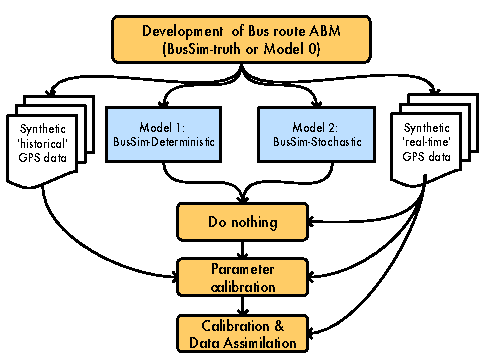
\includegraphics{Figures/framework14.pdf}
    \caption{Workflow\DIFaddbeginFL \DIFaddFL{. To begin with, an agent-based model of a bus network is created (BusSim-truth). This is used as a hypothetical real-world and means that }\textit{\DIFaddFL{full knowledge}} \DIFaddFL{of the system are available for the experiments (in reality this is impossible). Then two separate models are created that attempt to simulate the dynamics of the hypothetical real system.}\DIFaddendFL }
    \label{fig:workflow}
\end{figure}

The research approach in this paper starts with the development of a Markorvian ABM of bus route operation \DIFdelbegin \DIFdel{, }\DIFdelend that will be referred as \textit{BusSim-truth}, or \textit{Model 0} \DIFdelbegin \DIFdel{henceforth. }%DIFDELCMD < {%%%
\DIFdelend \DIFaddbegin \todo{Just call it BusSim-truth, not Model 0 as well, less confusing} \DIFadd{henceforth. }\DIFaddend BusSim-truth \DIFdelbegin %DIFDELCMD < } %%%
\DIFdel{is a }\DIFdelend \DIFaddbegin \DIFadd{is a hypothetical }\DIFaddend version of reality \DIFdelbegin \DIFdel{, because we predefine all the parameters of this model, and will use for generating }\DIFdelend \DIFaddbegin \DIFadd{and will be used to generate }\DIFaddend synthetic GPS data of bus locations with timestamps. Two sets of data will be generated\DIFdelbegin \DIFdel{, one is a '}\DIFdelend \DIFaddbegin \DIFadd{. The first represents `}\DIFaddend historical' GPS data, which \DIFdelbegin \DIFdel{is }\DIFdelend \DIFaddbegin \DIFadd{are }\DIFaddend essentially the outputs of multiple runs of the same BusSim-truth model with the same set of parameters. The GPS data will be slightly different each time \DIFdelbegin \DIFdel{we run the }\DIFdelend model because BusSim-truth is a stochastic and dynamic model. The second set of data \DIFdelbegin \DIFdel{is }\DIFdelend \DIFaddbegin \DIFadd{represent }\DIFaddend a single run of BusSim-truth, also using the same set of parameters, that \DIFdelbegin \DIFdel{we will use as a synthetic '}\DIFdelend \DIFaddbegin \DIFadd{will be used as synthetic `}\DIFaddend real-time' GPS data.

In practice, any model of the bus route is generally a simplification of reality. Models should be as simple as possible to fit a research purpose, because simple models are easier to implement and adjust, but we also want accurate predictions of bus locations. It is also very challenging to accurately model the dynamic changes of variables in practice using the limited \DIFdelbegin \DIFdel{, }\DIFdelend and uncertain data \DIFaddbegin \DIFadd{that are }\DIFaddend available. Therefore, we develop two simpler variations of BusSim compared to BusSim-truth and aim to use parameter calibration and DA to see whether these models can predict the bus location similar to the synthetic \DIFdelbegin \DIFdel{'}\DIFdelend \DIFaddbegin \DIFadd{`}\DIFaddend real-time' GPS data, as would happen were the model simulating a real system\DIFdelbegin \DIFdel{where limited, and uncertain, data were available}\DIFdelend . The two variations are: 
\DIFaddbegin \begin{itemize}
	\item \DIFaddend Model 1: BusSim-deterministic\DIFdelbegin \DIFdel{and Model 2: BusSim-stochastic. The deterministic model (Model 1) }\DIFdelend \DIFaddbegin \DIFadd{. This model }\DIFaddend evolves exactly the same way at similar situation, e.g. exactly the same number of passengers get on the bus when the time gap between buses are similar\DIFdelbegin \DIFdel{, versus the stochastic model (}\DIFdelend \DIFaddbegin \DIFadd{.}\todo{Minh: please rephrase the description of Model 1, I don't understand it} 
	\item \DIFaddend Model 2\DIFdelbegin \DIFdel{), which behaves slightly different at similar situations. }\DIFdelend \DIFaddbegin \DIFadd{: BusSim-stochastic. This model is stochastic, so behaves slightly differently in similar situations}\todo{Minh: another sentence about what the differences are (I think passenger arrival rate and traffic?}\DIFadd{. 
}\end{itemize}
\DIFaddend The models will be calibrated against the synthetic \DIFdelbegin \DIFdel{'}\DIFdelend \DIFaddbegin \DIFadd{`}\DIFaddend historical' GPS data and DA will be applied against the synthetic \DIFdelbegin \DIFdel{'}\DIFdelend \DIFaddbegin \DIFadd{`}\DIFaddend real-time' GPS data. Broadly, this experimental approach is known as the \DIFdelbegin \DIFdel{'}\DIFdelend \DIFaddbegin \DIFadd{`}\DIFaddend identical twin' experiment \citep{wang_data_2015}. The next section will describe this research methodology in more \DIFdelbegin \DIFdel{details}\DIFdelend \DIFaddbegin \DIFadd{detail}\DIFaddend . 

\DIFdelbegin %DIFDELCMD < \todo[inline]{[MK] I go with two models here: Determinisitic and Static models. It's important to note that BusSim-truth is both \textit{stochastic} and \textit{dynamic}, so both Model 1 and Model 2 would fail to predict what BusSim-truth has generated. I argue that this is similar to the practice and this is a good case of use for parameter calibration \& data assimilation!
%DIFDELCMD < 

%DIFDELCMD < However, the amount of stochasticity and dynamicity that we can deal with may be limited. I will need to find an effective range using experiments, but I reckon that it may be quite limited. 
%DIFDELCMD < 

%DIFDELCMD < Another option would be to include a 'Model 3' which is also dynamic and stochastic, similar to BusSim-truth, and calibrate it so that it would produce perfect results. But then it is quite unrealistic because in practice it is very challenging to make this Model 3 without knowing the inherent dynamics in the data. 
%DIFDELCMD < 

%DIFDELCMD <  What do you think?
%DIFDELCMD < } 
%DIFDELCMD < %%%
\DIFdelend \DIFaddbegin \todo[inline]{[MK] I go with two models here: Determinisitic and Static models. It's important to note that BusSim-truth is both \textit{stochastic} and \textit{dynamic}, so both Model 1 and Model 2 would fail to predict what BusSim-truth has generated. I argue that this is similar to the practice and this is a good case of use for parameter calibration \& data assimilation!

However, the amount of stochasticity and dynamicity that we can deal with may be limited. I will need to find an effective range using experiments, but I reckon that it may be quite limited. 

Another option would be to include a 'Model 3' which is also dynamic and stochastic, similar to BusSim-truth, and calibrate it so that it would produce perfect results. But then it is quite unrealistic because in practice it is very challenging to make this Model 3 without knowing the inherent dynamics in the data. 

 What do you think?

 [NM] : It's perfect as is as far as I can tell. If necessary we can just be honest about the limited range in the experiments, the paper still makes a novel contribution.
} 
\DIFaddend 

% !TEX root = BusSim.tex
\section{Methodology\label{s:method}}

This section describes the proposed methodology\DIFdelbegin \DIFdel{in this paper}\DIFdelend . It includes a subsection on the development of agent-based bus route operation model (\DIFdelbegin \DIFdel{BusSim) }\DIFdelend \DIFaddbegin \DIFadd{BusSim-truth) used to generate the synthetic data}\DIFaddend , a parameter calibration procedure, and a data assimilation algorithm to incorporate \DIFaddbegin \DIFadd{`}\DIFaddend real-time\DIFdelbegin \DIFdel{data into BusSim. }\DIFdelend \DIFaddbegin \DIFadd{' data into the two simulations (BusSim-deterministic and BusSim-stochastic). The source code for all of these models is available in full at }\url{XXXX}\DIFadd{.
}\DIFaddend 

\subsection{Notation}
\DIFaddbegin 

\DIFadd{The following notation will be used to formalise each of the simulation models:
}

\DIFaddend \label{s:Notation}
\begin{itemize}
    \item $dt$: Time interval ($s$)
    \item $t$: Current time ($s$ from 00:00:00)
    \item $N$: Number of buses
	\item $j$: Index of vehicle $(j=1..N)$
	\item $m$: Index of bus stop $(m=1..M)$
	\item $M$: Number of bus stops
	\item $c_j$: Current status of bus j (IDLE, MOVING, DWELLING or FINISHED)
	\item $a_j$: Acceleration rate of bus j ($m/s^2$)
	\item $v_j$: Current speed of bus j ($m/s$)
	\item $Occ_{j}$: Current occupancy of bus $j$ (number of passengers onboard)
	\item $H$: Scheduled headway ($s$)
	\item $C$: Bus capacity
	\item $V$: Traffic speed ($m/s$)
	\item $\delta_j$: The scheduled dispatch time of bus $j$ from the first stop
	\item $t^a_{j,m}$: Arrival time of bus $j$ at stop $m$
	\item $t^d_{j,m}$: The moment when bus $j$ can leave stop $m$ after passenger boarding and alighting (or $Leave\_stop\_time$)
    \item $D_{j,m}$: Dwell time of bus $j$ at stop $m$ for passenger boarding and alighting
	\item $\theta_1,\theta_2,\theta_3$: Parameters set for estimating $D_{j,m}$
	\item $B_{j,m}$: Number of boarding passenger to bus $j$ at stop $m$
	\item $A_{j,m}$: Number of alighting passenger from bus $j$ at stop $m$
	\item $Arr_m$: Arrival rate of passengers to stop $m$ per second
	\item $Dep_m$: Departure rate of passengers from stop $m$

\end{itemize}

\subsection{A \DIFaddbegin \DIFadd{hypothetical }\DIFaddend version of reality: \DIFdelbegin \DIFdel{Pseudo-truth model of bus route (}\DIFdelend BusSim-truth\DIFdelbegin \DIFdel{)}\DIFdelend }

\DIFdelbegin \DIFdel{As previous mentioned in the Section \ref{s:Intro}, the first step }\DIFdelend \DIFaddbegin \DIFadd{The first step in the proposed workflow }\DIFaddend is to develop an agent-based bus route model that will be used to generate synthetic GPS data \DIFaddbegin \DIFadd{for each bus on the route}\DIFaddend , which will be referred as BusSim-truth \DIFdelbegin \DIFdel{or Model 0 }\DIFdelend henceforth. BusSim-truth is a stochastic and dynamic model with predefined parameters. It is stochastic because the number of boarding passengers is \DIFdelbegin \DIFdel{random}\DIFdelend \DIFaddbegin \DIFadd{drawn from a randomly distribution}\DIFaddend , and dynamic because it parameters gradually change over time. The \DIFaddbegin \DIFadd{level of }\DIFaddend stochasticity and dynamicity \DIFdelbegin \DIFdel{level }\DIFdelend in BusSim-truth can also be adjusted to represent bus route systems where conditions are largely stable or volatile over time.

BusSim-truth is an agent-based model with two classes of agents: Bus and bus stop. Table \ref{tab:Agents} lists those classes with their parameters.  

\DIFaddbegin \todo[inline]{We should consider moving a lot of this to an appendix and writing an ODD document. I'm tempted to leave it as it is because we're not going for an agent-based modelling journal (otherwise we'd have to write ODD) and there isn't so much detail that it drowns out the rest. Alison what do you think?}

\DIFaddend \begin{table}[htbp]
  \centering
  \caption{Type of agents and their parameters in BusSim-truth}
    \begin{tabular}{rll}
    \toprule
    \multicolumn{1}{l}{\textbf{Class}} & \textbf{Parameter} & \textbf{Description} \\
    \midrule
    \multicolumn{1}{l}{Bus} & BusID  & Unique ID of the bus agent \\
          & Acceleration & The acceleration value in $m/s^2$ if the bus needs to accelerate \\
          & StoppingTime & Deadtime due to door opening and closing if the bus has to stop \\
          & Visited & List of visited bus stops \\
          & States & Whether the bus is idle, moving, dwelling or finished \\
          & Trajectory & GPS coordinates of bus locations \\
    \midrule
    \multicolumn{1}{l}{BusStop} & bus stopID & Unique ID of the bus stop \\
          & Position & Distance from the first stop \\
          & $Arr_m$ & Passengers arrived to the stop per second \\
          & $Dep_m$ & Percentage of onboard passengers alight at the stop \\
          & Arrival\_time & Store actual arrival time of buses at the stop \\
          & GeoFence & A circle area to identify whether the bus is at the bus stop \\
    \bottomrule
    \end{tabular}%
  \label{tab:Agents}%
\end{table}%

\DIFdelbegin \DIFdel{A part from }\DIFdelend \DIFaddbegin \DIFadd{In addition to }\DIFaddend these parameters, BusSim-truth also use global parameters which are generally fixed through out the simulation. Examples of those parameters are the time interval $dt$, the number of stop $N$, and other parameters that can found in the Notation section (\ref{s:Notation})\DIFdelbegin \DIFdel{of this paper}\DIFdelend .

Figure \ref{fig:BusSim_flowchart} illustrates the \DIFdelbegin \DIFdel{work flow of }\DIFdelend \DIFaddbegin \DIFadd{workflow for }\DIFaddend BusSim-truth. At each current time step $t$, \DIFdelbegin \DIFdel{we loop through }\DIFdelend each Bus agent \DIFdelbegin \DIFdel{to first check }\DIFdelend \DIFaddbegin \DIFadd{checks }\DIFaddend whether the next time step would be or would pass \DIFaddbegin \todo{`would be or would pass' ? - rephrase, I don't understand} \DIFaddend the vehicle's scheduled dispatch time $\delta_j$ or not. If $t>\delta_j$, we then check whether the bus is on the road (Status equals $MOVING$), or at a stop for passenger dwelling (Status equals $DWELLING$), or has finished its service (Status equals $FINISHED$), otherwise the bus remains $IDLE$. 

If the status is $MOVING$, we first check whether the bus is at a bus stop, by comparing the $GeoFence$ area of each bus stop agent with the bus' location. If the bus is not approaching a bus stop, its current speed $v_j$ will be compared with the surrounding traffic speed $V$. If $v_j<V$, we assume that the bus will speed up with an acceleration rate $a_j$, thus we have: 
\DIFdelbegin %DIFDELCMD < 

%DIFDELCMD < %%%
\DIFdelend \begin{equation}
    v_j^{t} = v_j^{t-dt} + a_j \cdot dt
\end{equation}

\DIFdelbegin \DIFdel{Thus }\DIFdelend \DIFaddbegin \DIFadd{Therefore }\DIFaddend for the next time step, the bus will cover a distance of: 
\DIFdelbegin %DIFDELCMD < 

%DIFDELCMD < %%%
\DIFdelend \begin{equation}
    S_j^t = S_j^{t-dt} + v_j^t \cdot dt
\end{equation}

If the speed already matches the traffic speed $V$, the bus will maintain the same speed. Or else if the bus is approaching a bus stop, the system will first check if the stop is the last stop. If it is the last stop, then the bus' status will be changed to $FINISHED$ and bus speed is changed to zero. If it is not the last stop, the system will change the status of agent Bus $j$ to $DWELLING$ and its speed to zero. The number of boarding and alighting passenger from the bus $j$, and the time that it will leave the stop are estimated as follows.  

\DIFdelbegin %DIFDELCMD < \begin{figure}[htbp]
%DIFDELCMD <     %%%
\DIFdelendFL \DIFaddbeginFL \begin{figure}[ht]
    \DIFaddendFL \centering
    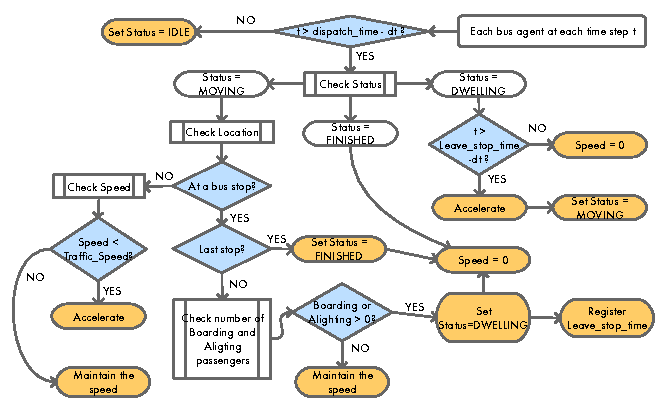
\includegraphics{Figures/bussim_flowchart6.pdf}
    \caption{Flowchart of \DIFdelbeginFL \DIFdelFL{BusSim}\DIFdelendFL \DIFaddbeginFL \DIFaddFL{BusSim-truth.}\DIFaddendFL }
    \label{fig:BusSim_flowchart}
\end{figure}

The number of boarding passenger is proportional to the time gap between the current time (when Bus $j$ approaches the bus stop $m$) and the last time any bus visits the bus stop $m$\DIFdelbegin \DIFdel{. 
    }%DIFDELCMD < 

%DIFDELCMD <     %%%
\DIFdelend \DIFaddbegin \DIFadd{:     
    }\DIFaddend \begin{equation}
        B_{j,m} = \nint{Po(Arr_m \cdot (t^a_{j+1,m}-t^a_{j,m}) } \quad | \quad B_{j,m}\in\mathbb{N}
        \label{eq:Boarding_est}
    \end{equation}

Equation \ref{eq:Boarding_est} shows that the number of boarding passengers is estimated using a stochastic Poisson process. A Poisson process is widely adopted in literature to estimate the count of passengers waiting at a public transport stop \citep{toledo2010mesoscopic,cats2010mesoscopic}. Extensions of this stochastic process \DIFdelbegin \DIFdel{has }\DIFdelend \DIFaddbegin \DIFadd{have }\DIFaddend been introduced, such as non-homogeneous Poisson process \citep{kieu2018stochastic}, where the arrival rate is time-dependent, but for simplicity we adopt a homogeneous Poisson process for this paper. Equation \ref{eq:Boarding_est} makes the BusSim-truth model stochastic, because there is randomness in the way the Poisson process \DIFdelbegin \DIFdel{generate }\DIFdelend \DIFaddbegin \DIFadd{generates }\DIFaddend a number. For more details on the number generation process using stochastic Poisson process (e.g. thinning algorithm), interested readers may refer to \citet{lewis1979simulation}. \DIFdelbegin %DIFDELCMD < 

%DIFDELCMD < %%%
\DIFdelend The number of boarding passengers is also limited by the available capacity of the bus\DIFdelbegin %DIFDELCMD < 

%DIFDELCMD <     %%%
\DIFdelend \DIFaddbegin \DIFadd{:
    }\DIFaddend \begin{equation}
        B_{j,m} = \text{max} \big( B_{j,m}, C - Occ_m )   \big)
        \label{eq:Boarding_est}
    \end{equation}

The number of alighting passengers is proportional to the number of passenger on board (bus occupancy) and the departure rate at the stop $m$.  For simplicity, we assume that $A_{j,m}$ is the product between the departure rate from bus stop $m$ and the current bus occupancy (the number of passenger on board leaving the last stop)\DIFdelbegin \DIFdel{. 
}%DIFDELCMD < 

%DIFDELCMD <     %%%
\DIFdelend \DIFaddbegin \DIFadd{: 
    }\DIFaddend \begin{equation}
        A_{j,m} = \nint{Dep_m \cdot Occ_{j,m-1}} \quad | \quad A_{j,m}\in\mathbb{N}
    \end{equation}

\DIFdelbegin \DIFdel{Now to }\DIFdelend \DIFaddbegin \DIFadd{To }\DIFaddend estimate the amount of time that bus will have to stay at the bus stop $m$ for passenger boarding and alighting, a.k.a. \textit{dwell time} $D_{j,m}$, we adopt the approach in \citet{bertini2004modeling} and the TCQSM \citep{kfh2013transit}\DIFdelbegin \DIFdel{. 
}%DIFDELCMD < 

%DIFDELCMD < %%%
\DIFdelend \DIFaddbegin \DIFadd{:
}\DIFaddend \begin{equation}
D_{j,m} = \theta_1 + \theta_2 \times B_{j,m} + \theta_3 \times A_{j,m} 
\label{eq:dwell_time}
\end{equation}
\DIFdelbegin %DIFDELCMD < 

%DIFDELCMD < %%%
\DIFdelend The parameter set [$\theta_1,\theta_2,\theta_3$] represents the time spent for passenger boarding, alighting, and a fixed value for vehicle stopping and starting, respectively. Equation \ref{eq:dwell_time} is the formulation for a single-door bus system, where boarding and alighting occurs sequentially. 

The departure time of bus $j$ from stop $m$ is calculated from the arrival time $t^a_{j,m}$ plus the time spent at stops for passenger boarding and alighting, or in other words the dwell time $D_m$\DIFdelbegin \DIFdel{. 
}%DIFDELCMD < 

%DIFDELCMD < %%%
\DIFdelend \DIFaddbegin \DIFadd{:
}\DIFaddend \begin{equation}
	 t^d_{j,m} = t^a_{j,m} + D_{j,m}
\end{equation}
\DIFdelbegin %DIFDELCMD < 

%DIFDELCMD < %%%
\DIFdelend In BusSim, the bus $j$ is only allowed to leave the bus $m$ at time $t^d_{j,m}$, so this is also called the $Leave\_stop\_time$, as can be seen in the Figure \ref{fig:BusSim_flowchart}. 

If the status of bus $j$ is $DWELLING$, it is at a stop for passenger boarding and alighting. We then check if the next time step would be larger or equal to the leave stop time $t^d_{j,m}$. If it would, then the bus would start accelerate to leave the stop, otherwise it would stay for at least another time interval. Finally, if the status of the bus is $FINISHED$, then we would do nothing. The modelling process then moves to the next Bus agent until the last Bus, then the whole model moves to the next time step until the last time step. 

BusSim-truth also \DIFdelbegin \DIFdel{assume }\DIFdelend \DIFaddbegin \DIFadd{assumes }\DIFaddend that parameters dynamically change over time \DIFdelbegin \DIFdel{, }\DIFdelend by introducing an additional parameter $\xi$ to represent the change in passenger demand or surrounding traffic speed. For simplicity, we assume that a single, deterministic parameter $\xi$ can model these dynamic changes. In practice, it is possible, and more desirable\DIFaddbegin \DIFadd{, }\DIFaddend to use a time-dependent value of $\xi$ such that dynamic change is better captured, and multiple $\xi$ to model different changes. $\xi>0$ represents an increase in passenger demand and traffic speed, and $\xi<0$ represents otherwise. In this paper, the change in passenger demand or traffic speed is modelled as: 
    \DIFdelbegin %DIFDELCMD < 

%DIFDELCMD <     %%%
\DIFdelend \begin{align}
        V = V \cdot \big( 1 - \frac{t}{T} \cdot \frac{100}{\xi} \big) \\
        Arr_m = Arr_m \cdot (1 - \frac{t}{T} \cdot \frac{100}{\xi}
        \label{eq:dynamic_bussim}
    \end{align}
\DIFdelbegin %DIFDELCMD < 

%DIFDELCMD < %%%
\DIFdelend A positive value of $\xi$ in Equation \ref{eq:dynamic_bussim} gradually reduces the surrounding traffic speed $V$ and \DIFdelbegin \DIFdel{increase }\DIFdelend \DIFaddbegin \DIFadd{increases }\DIFaddend the arrival rate $Arr_m$, which would lead to more bus delays and \DIFdelbegin \DIFdel{congestions}\DIFdelend \DIFaddbegin \DIFadd{congestion}\DIFaddend . 

\subsection{\DIFdelbegin \DIFdel{Simpler models }\DIFdelend \DIFaddbegin \DIFadd{Verification }\DIFaddend of \DIFdelbegin \DIFdel{bus routes}\DIFdelend \DIFaddbegin \DIFadd{BusSim-truth}\DIFaddend }

\DIFaddbegin \todo[inline]{I suggested showing that the BusSim-truth model generates realistic-looking data by comparing the outputs to some real data that Minh has from Brisbane. Alison do you think this new section that I'm proposing is necessary? My concern is that someone could say that if BusSim-truth does not generate realistic-looking data then the who paper is fundamentally flawed. Before deciding, read the first bullet point in the next section as it might clarify what I'm on about. 

If you don't think that this is necessary then we can leave it out, it will add a fair few words and might just get the reviewers asking more questions.}

\subsection{\DIFadd{Simpler models of bus routes: BusSim-deterministic and BusSim-stochastic}}

\DIFaddend As described in Section \ref{s:problem}, we use BusSim-truth to generate two sets of data.  

\begin{itemize}
    \item Synthetic \DIFdelbegin \DIFdel{'}\DIFdelend \DIFaddbegin \DIFadd{`}\DIFaddend historical' GPS data: This dataset is a collection of Bus agents' locations at every time step for a hundred of runs of BusSim-truth, using the same predefined set of parameters. This is \DIFdelbegin \DIFdel{mimicking a }\DIFdelend \DIFaddbegin \DIFadd{mimics the }\DIFaddend collection of historical \DIFaddbegin \DIFadd{bus }\DIFaddend GPS data in practice, where the bus location \DIFdelbegin \DIFdel{can be slightly to significantly }\DIFdelend \DIFaddbegin \DIFadd{will be }\DIFaddend different on each day due to the stochasticity in the bus operation system \DIFaddbegin \DIFadd{and the surrounding environment}\DIFaddend . This dataset will be used to calibrate \DIFaddbegin \DIFadd{the }\DIFaddend simpler bus route ABMs (Figure \ref{fig:workflow}). 
    \item Synthetic \DIFdelbegin \DIFdel{'}\DIFdelend \DIFaddbegin \DIFadd{`}\DIFaddend real-time' GPS data: this dataset includes the locations of all Bus agents for a single run of the BusSim-truth for every time step. This dataset will be used in the DA algorithm \DIFdelbegin \DIFdel{implementation and in the evaluation of calibration and DA on each variation of bus route ABMs}\DIFdelend \DIFaddbegin \DIFadd{as a hypothetical proxy for data that are being generated by the real world in real-time}\DIFaddend . 
\end{itemize}

Each record in the synthetic \DIFdelbegin \DIFdel{'}\DIFdelend \DIFaddbegin \DIFadd{`}\DIFaddend historical' GPS data or \DIFdelbegin \DIFdel{'}\DIFdelend \DIFaddbegin \DIFadd{`}\DIFaddend real-time' data, produced by BusSim-truth, is called an \textit{observation vector}. The vector contains all of the observations made from the \DIFdelbegin \DIFdel{'}\DIFdelend \DIFaddbegin \DIFadd{`}\DIFaddend real world' (in this case the BusSim-truth)\DIFdelbegin %DIFDELCMD < 

%DIFDELCMD < %%%
\DIFdelend \DIFaddbegin \DIFadd{:
}\DIFaddend \begin{equation}
  O  = \left[ \begin{array}{ccccccc}
s_1, s_2, \dots s_N
\end{array} \right] \quad
\end{equation} 

\DIFdelbegin \DIFdel{The observation vector contains the location of all buses in the system at time step $t$, and that is why $O$ is called synthetic GPS data. }\DIFdelend We develop two variations of the bus route model to be calibrated and incorporated with this observation vector to provide predictions of bus locations. 

\begin{enumerate}
    \item Model 1 - Static and Deterministic BusSim: The first model is a static and deterministic variation of \DIFdelbegin \DIFdel{BusSim}\DIFdelend \DIFaddbegin \DIFadd{BusSim-truth}\DIFaddend . This model is static because we change Equation \ref{eq:Boarding_est} into a static estimation of the number of boarding passengers: 
        \DIFdelbegin %DIFDELCMD < 

%DIFDELCMD <         %%%
\DIFdelend \begin{equation}
        B_{j,m} = \nint{Arr_m \cdot (t^a_{j+1,m}-t^a_{j,m}) } \quad | \quad B_{j,m}\in\mathbb{N}
        \label{eq:Boarding_est_static}
        \end{equation}
    \DIFdelbegin %DIFDELCMD < 

%DIFDELCMD <     %%%
\DIFdelend Model 1 is also static because none of its parameters will be changed over time. 

    \item Model 2 - Static and Stochastic BusSim: The second model is a static, but stochastic variation of \DIFdelbegin \DIFdel{BusSim. The }\DIFdelend \DIFaddbegin \DIFadd{BusSim-truth. }\DIFaddend Equation \ref{eq:Boarding_est} is adopted to \DIFdelbegin \DIFdel{enable }\DIFdelend \DIFaddbegin \DIFadd{allow }\DIFaddend stochasticity in the model, but the model is still static \DIFdelbegin \DIFdel{, }\DIFdelend because none of its parameters will be changed over time. 

\end{enumerate}


\subsection{Parameter calibration of Model 1 and 2}
\label{s:calibration}

Most agent-based models have a large number of parameters that are essential for their performance. Recall that a dynamic simulator may be written in the form $Y = f(X)$ where $X$ includes all the model parameters. For BusSim models (Model 1 and Model 2), vector $X$ contains the arrival rate $Arr_m$, departure rate $Dep_m$ at each stop $m$, and the traffic speed $V$. 
\DIFdelbegin %DIFDELCMD < 

%DIFDELCMD < %%%
\DIFdelend \begin{equation}
  X  = \left[ \begin{array}{ccc}
Arr_m & Dep_m & V  
\end{array} \right] \quad m=1..M 
\label{eq:X}
\end{equation} 

Adjusting these parameters by hand is tedious and impossible for real-time applications. This subsection describes an automatic parameter calibration process, based on the Cross-Entropy Method (CEM) \citep{rubinstein1999cross} for optimising \DIFdelbegin \DIFdel{parameters of BusSim. 
}\DIFdelend \DIFaddbegin \DIFadd{the parameters of the two simple BusSim models. }\todo{Why was CEM chosen over any of the other parameter optimisation approaches that are commonly used?}

\DIFaddend CEM is a population-based Monte Carlo learning algorithm to combinatorial multi-extremal optimisation and importance sampling. It originated from the field of rare event simulation, where even small probabilities need to be estimated. In principle, CEM develops a \textit{probability distribution} over possible solutions for the optimal parameters of the model. New solution candidates are drawn from this distribution and are evaluated. The best candidates are then selected to form a new improved probability distribution of the optimal parameters, until certain criteria are met. \DIFdelbegin \DIFdel{Interested }\DIFdelend \DIFaddbegin \DIFadd{The interested }\DIFaddend reader may refer to the Appendix\DIFdelbegin \DIFdel{A }\DIFdelend \DIFaddbegin \DIFadd{~\ref{appendix:cem} }\DIFaddend for more detailed account of the CEM. 

\DIFaddbegin \todo[inline]{As this paper isn't about calibrating ABMs, should all of the next bit go to the appendix? I think it's overkill. (I've skipped it for now as I want to get on to the PF etc).}

\DIFaddend The parameter calibration is an optimisation problem to minimise some performance index $PI(X)$ over all $X \in \mathbb{R}^k$. Here a solution $X= (X_1,X_2,...,X_k)$ denotes a set of parameters of the model under consideration and $k$ denotes the number of dimension in this set (see Equation \ref{e:statespace1}). Let $X_*$ denote the optimal solution, or the best set of model parameters that we want to find, that is:

\begin{equation}
    X_* = \text{argmin} \quad PI(X), \quad X \in \mathbb{R}^n
\end{equation}

The above objective function is equivalent to finding $X_*$ such that $PI(X_*) \leq PI(X) \quad \forall X \in \Pi$, where $\Pi$ is a constrained parameter space such that $\Pi \in \mathbb{R}^k$. The performance index $PI(X)$ is generally the difference between model output and observed data. The complexity of this problem comes from the stochasticity of BusSim, where the same solution $X$ may yield different realisation $PI(X)$. To reduce this stochastic effect, it is necessary to run the (stochastic) model multiple times, and also evaluate the simulation outputs against a compilation of observed data from multiple days or instances. Let $K_I$ be the number of replications required for each model evaluation and $K_O$ be the number of instances in the observed data, we can derive a more detailed objective function of the parameter calibration problem: 

\begin{align}
    \text{min} \ PI(X) = \frac{1}{N \cdot T} \sum_{t=1}^T \sum_{n=1}^N \Bigg[ \bigg|  \frac{1}{K_I} \sum^{K_I}  s_{j,i,t}^{SIM}  - \frac{1}{K_O} \sum^{K_O}  s_{j,o,t}^{OBS} \bigg| + \nonumber \\
    \bigg| \sqrt{\frac{\sum^{K_I} \big( s_{j,i,t}^{SIM} - \hat{s}_{j,i,t}^{SIM} \big)^2}{K_I-1}}  - \sqrt{\frac{\sum^{K_O} \big( s_{j,o,t}^{OBS} - \hat{s}_{j,o,t}^{OBS} \big)^2}{K_O-1}} \bigg|   \Bigg]
    \label{eq:objective_function}
\end{align}

Where $N$ is the number of buses, $T$ is the number of time steps, $s_{j,i,t}^{SIM}$ is the location of simulated bus agent $j$ at time $t$ for the replication $i$, and similarly $s_{j,o,t}^{OBS}$ is the synthetic observed location of bus $j$ at time $t$ for the instance $o$. The objective function in Equation \ref{eq:objective_function} can be seen as the sum of the difference in mean location and standard deviation of locations at each time step for each bus and each replication/instance between simulated outputs and synthetic observed data. We want to evaluate the difference in not just the mean but also the standard deviation of bus locations because the system under study is stochastic, so it is not just the mean but also the spread of bus locations over multiple instances are important. 

The proposed objective function is solved using CEM. The Appendix A provides more details and also provides a pseudo-code of this method. 

\subsection{Data Assimilation using Particle Filter (PF)}

Recall from Section \ref{s:problem} that we can formulate an ABM as a state-space model $Y_t = f(Y_{t-1},X,t) + \epsilon_k$ and use data assimilation (DA) to dynamically optimise this model with up-to-date data. \DIFdelbegin \DIFdel{State-space }\DIFdelend \DIFaddbegin \DIFadd{The state-space }\DIFaddend model is Markovian, and is represented by a state-space vector $S$, which contains all information of the current state of each agent in the model\DIFdelbegin \DIFdel{. 
}%DIFDELCMD < 

%DIFDELCMD < %%%
\DIFdelend \DIFaddbegin \DIFadd{: 
}\DIFaddend \begin{equation}
  S  = \left[ \begin{array}{ccccccc}
c_j^t & s_j^t & v_j^t & Occ_j^t & Arr_m & Dep_m & V  
\end{array} \right] \quad \forall j,m \quad t<T
\label{eq:state_vector}
\end{equation} 

The state-space vector $S$ \DIFdelbegin \DIFdel{should contain all }\DIFdelend \DIFaddbegin \DIFadd{must contain all of }\DIFaddend the information that \DIFdelbegin \DIFdel{would help identify }\DIFdelend \DIFaddbegin \DIFadd{identifies }\DIFaddend the current state of the \DIFdelbegin \DIFdel{system, and be ready to project }\DIFdelend \DIFaddbegin \DIFadd{modelled system, allowing it to be projected }\DIFaddend forward to the next time step. Thus vector $S$ is usually much longer than the observation vector $O$. \DIFdelbegin \DIFdel{It also contains information in $O$ because some of the information in the state vector may be observable, such as bus location. Vector }\DIFdelend $S$ also contains the parameter vector $X$, so that \DIFdelbegin \DIFdel{we can also dynamically calibrate the model }\DIFdelend \DIFaddbegin \DIFadd{the model can be dynamically calibrated }\DIFaddend with new data \DIFaddbegin \DIFadd{-- this is essential in dynamic situations where parameter values change over time}\DIFaddend . This approach is often refered as dynamic calibration in literature \citep{eicker2014calibration}.

\DIFaddbegin \todo{This is very similar to my ERC application :-) WHich is fine, I'm delighted that you can use it, but just make sure it's been paraphrased a bit.}\DIFaddend Data Assimilation (DA) often refers to a suite of statistical methods to incorporate up-to-date data to adjust the state of a running model to better represent the current state of the system under study \citep{ward_dynamic_2016}. DA was born out of data scarcity, where observation data are spatio-temporally sparse and insufficient to describe the system. Notwithstanding the proliferation of new data sources, insufficient data is still a major problem in research. The bus location prediction that being tackled in this paper is \DIFdelbegin \DIFdel{one of the }\DIFdelend \DIFaddbegin \DIFadd{a }\DIFaddend clear example, where the number of future boarding and alighting passengers are unknown in real time. DA algorithms fills in the spatio-temporal gaps in the observed data by running a model forward in time until new observed data are available. This is typically called the \textit{predict} step in DA algorithms. After the predict step, DA has an estimate of the current system state and its uncertainty (which is often referred as the \DIFdelbegin \DIFdel{'}\DIFdelend \DIFaddbegin \DIFadd{`}\DIFaddend prior' in Bayesian literature). The next step is typically called the \textit{update} step, where new observations and uncertainty are used to update the current step estimates. The result is often referred as the \DIFdelbegin \DIFdel{'}\DIFdelend \DIFaddbegin \DIFadd{`}\DIFaddend posterior' in Bayesian literature, and should be the best guest of the system state from both the observations and model\DIFaddbegin \todo{This explanation of DA is fine, but I think it could do with a diagram to show model iterations, the DA window, etc. I'm going to do one of these for Kevin's paper anyway so will do one for this paper too}\DIFaddend .   

There are several DA algorithms in literature, ranging from the simple Kalman Filter \citep{meinhold1983understanding} to more advanced extensions, including extended, ensemble and unscented Kalman Filter \citep{jazwinski_stochastic_1970, evensen_ensemble_2003,wan_unscented_2002}. These algorithms generally aim to extend the original Kalman Filter by relaxing the assumption of linearity and introducing methods to work with non-linear models. However, they may not be the most suitable candidate to incorporate data into ABMs because of two reasons. First, ABMs is driven by a large number of interacting agents with goals, history and behavioural rules. As a result, they lack of an analytic structure and complicate the implementation of conventional Kalman Filter and its extensions, which have been developed to work with differential or difference equations \citep{wang_data_2015}. Second, although the assumption of linearity has been relax, these extensions of Kalman Filter still assume that the noise in the model estimation being Gaussian. 

There is a Bayesian filtering method that has been designed to work with non-linear, non-Gaussian and models without analytical structure, that is Particle Filter (PF). \DIFaddbegin \DIFadd{A }\DIFaddend PF is a Bayesian state estimation method. The key idea is to approximate a posterior distribution by a set of samples or particles, drawn from this distribution. Each particle is a concrete hypothesis of the true system state. The set of particle approximates the posterior distribution. PF is best described as a nonparametric Bayes filter because it develops the belief not in analytical form but using a finite number of samples. 

Hypotheses of the system state at time $t$ is represented by a set $P_t$ of $N_P$ weighted random particles: 
\DIFdelbegin %DIFDELCMD < 

%DIFDELCMD < %%%
\DIFdelend \begin{equation}
    P_t =  \{  \langle X_t^{\nint{i}}, w_t^{\nint{i}} \rangle \ | \ i=1,...,N_P \}
\end{equation}
\DIFdelbegin %DIFDELCMD < 

%DIFDELCMD < %%%
\DIFdelend where $X_t^{\nint{i}}$ is the state vector of the \textit{i}-th particle and $w_t^{\nint{i}}$ is the corresponding weight. Weights are non-zero, and sum over all weights is 1. The core idea of \DIFaddbegin \DIFadd{the }\DIFaddend PF is to update and maintain this set of particles given model outputs and observations. \DIFaddbegin \DIFadd{A }\DIFaddend PF recursively estimates the particle set $P_t$ based on the estimate $P_{t-1}$ at the previous time step, and the observation. The PF algorithm can be briefly described in three steps: 

\begin{enumerate}
    \item \textbf{Predict:} Generate the next set of particles $\hat{P}_t$ from the previous set $P_{t-1}$. This represents the \textit{prior} distribution to describe how the system state evolves. 
    \item \textbf{Importance Weighting:} Compute the importance weight $w_t^{\nint{i}}$ for each particle in $P_t$. This is equivalent to the \DIFdelbegin \DIFdel{'}\DIFdelend \DIFaddbegin \DIFadd{`}\DIFaddend Update' step in Kalman Filter, and will give us the \textit{posterior} distribution 
    \item \textbf{Resampling:} This step has no analogous step in Kalman Filter and its extensions. The resampling step creates a new set of particles from the current set with replacement. The likelihood to draw a particle is proportional to its weight. We adopt Sample Importance Resampling, a popular bootstrap systematic resampling in PF literature \citep{wang_data_2015, carrassi_data_2018}.
\end{enumerate}

The PF is applied to Model 1 and Model 2 using up-to-date data from the synthetic \DIFdelbegin \DIFdel{'}\DIFdelend \DIFaddbegin \DIFadd{`}\DIFaddend real-time' GPS data. Interested reader may refer to the Appendix B for a more formal and more details explaination of the applied PF algorithm in this paper. \DIFaddbegin \todo{PF description is clear, concise, and shows an appreciation for how the method has been formalised. I like it a lot :-)}
\DIFaddend 



%DIF >  !TEX root = BusSim.tex
\section{Numerical experiment}
\label{s:experiments}
\subsection{Experiment set up}

BusSim-truth simulates a hypothetical bus route with 20 bus stops and the length between two bus stops is 2000m\DIFaddbegin \todo{Need to justify this choice of number of stops and distance. Refer to Brisbane data? 2km is probably too big for the UK, but that doesn't matter}\DIFaddend . Buses are dispatched every 5 minutes from the first bus stop. We will simulate for a total of 100 minutes. We adopt the parameter set [$\theta_1,\theta_2,\theta_3$] from \citet{bertini2004modeling}. The bus acceleration rate is assumed as 3 $m/s^2$. The surrounding traffic speed is initially set as 14 $m/s$\DIFaddbegin \todo{These numbers need to be justified as well}\DIFaddend .

The arrival rate at stop $m$ is randomly generated from an uniform distribution between the minimum and maximum passenger arrival rate [$minDemand, maxDemand$] = [0.5, 1]. This is equivalent to 0.5 to 1 passenger arriving at the bus stop each second.  
\DIFdelbegin %DIFDELCMD < 

%DIFDELCMD < %%%
\DIFdelend \begin{equation}
    Arr_m = \mathcal{U} (minDemand, maxDemand) \quad m = 1,...,M
    \label{eq:arrival_rate}
\end{equation}

The departure rate is also generated from an uniform distribution, but also ordered non-decreasingly to represent the fact that more passengers alight at the end of the route than at the beginning. The departure rate at the last stop (stop M) is set as 1 to let every remaining passengers to alight the bus at the last stop. 
\DIFdelbegin %DIFDELCMD < 

%DIFDELCMD < %%%
\DIFdelend \begin{equation}
    Dep_m =  ordered \ (\mathcal{U} (0.05, 0.5)), \quad Dep_M = 1 \& \quad m = 1,...,M
     \label{eq:departure_rate}
\end{equation}

The dynamic parameter $\xi$ is set to be equal 5, which means that the passenger arrival rate will gradually increase to be 5\% more than the original value generated in Equation \ref{eq:arrival_rate}, and the surrounding traffic speed will also gradually reduce to be 5\% less than the original value.  

This same set of parameters is used to generate both the synthetic \DIFdelbegin \DIFdel{'}\DIFdelend \DIFaddbegin \DIFadd{`}\DIFaddend historical' and \DIFdelbegin \DIFdel{'}\DIFdelend \DIFaddbegin \DIFadd{`}\DIFaddend real-time' GPS data. Figure \ref{fig:historical_realtime} \DIFaddbegin \todo{Minh: one thing that the data don't show are bus bunching or leapfrogging. How difficult would it be to configure the BusSim-truth in such a way as to generate these features? That would be a nice test of the PF. Maybe as a subsequent section: `now look what happens when we apply it to a really complicated system'.} \DIFaddend shows a space-time diagram of synthetic bus trajectories from the \DIFdelbegin \DIFdel{'}\DIFdelend \DIFaddbegin \DIFadd{`}\DIFaddend historical' and \DIFdelbegin \DIFdel{'}\DIFdelend \DIFaddbegin \DIFadd{`}\DIFaddend real-time' GPS data. 

\begin{figure}[htb]
    \centering
    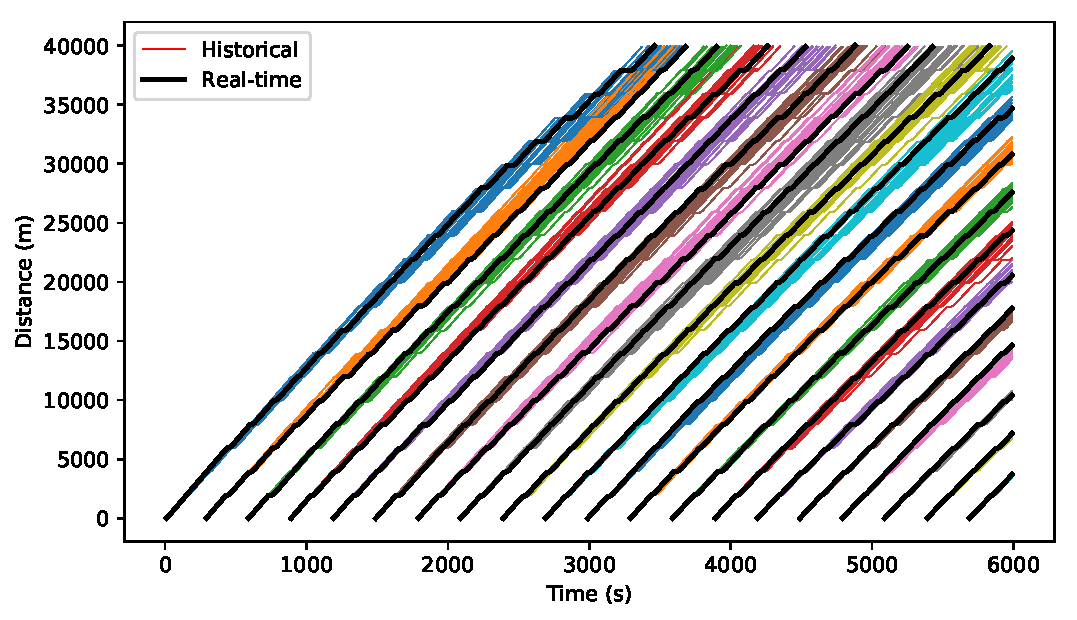
\includegraphics[width=\textwidth]{Figures/Fig_spacetime_dynamic.pdf}
    \caption{Synthetic \DIFdelbeginFL \DIFdelFL{'}\DIFdelendFL \DIFaddbeginFL \DIFaddFL{`}\DIFaddendFL historical' versus \DIFdelbeginFL \DIFdelFL{'}\DIFdelendFL \DIFaddbeginFL \DIFaddFL{`}\DIFaddendFL real-time' GPS bus location data\DIFaddbeginFL \DIFaddFL{. Each diagonal line shows the distance from the start that a single bus has travelled over time, with different colours representing different buses.}\DIFaddendFL }
    \label{fig:historical_realtime}
\end{figure}

Each coloured line shows the trajectory of one bus in the \DIFdelbegin \DIFdel{'}\DIFdelend \DIFaddbegin \DIFadd{`}\DIFaddend historical' GPS data. As the BusSim-truth model is stochastic, there is some random difference between the trajectories. This is similar to the reality where buses operate slightly \DIFdelbegin \DIFdel{different }\DIFdelend \DIFaddbegin \DIFadd{differently }\DIFaddend on multiple days. The bold black lines are another instance of bus trajectory that we consider as the \DIFdelbegin \DIFdel{'}\DIFdelend \DIFaddbegin \DIFadd{`}\DIFaddend real-time' GPS data. Recall that the Model 1 and Model 2 will be calibrated against the \DIFdelbegin \DIFdel{'}\DIFdelend \DIFaddbegin \DIFadd{`}\DIFaddend historical' data and evaluated against the \DIFdelbegin \DIFdel{'}\DIFdelend \DIFaddbegin \DIFadd{`}\DIFaddend real-time' data. Figure \ref{fig:historical_realtime} shows that even though \DIFdelbegin \DIFdel{'}\DIFdelend \DIFaddbegin \DIFadd{`}\DIFaddend real-time' data should \DIFaddbegin \DIFadd{... }\todo{?? something missing here}
\DIFaddend 

\subsection{\DIFdelbegin \DIFdel{Doing nothing scenario}\DIFdelend \DIFaddbegin \DIFadd{Base Scenario: no calibration}\DIFaddend }

This scenario aims to evaluate the prediction results from Model 1 and Model 2 \textit{without} calibrating their parameters or doing data assimilation. The two models are implemented using random parameters generated from Equation \ref{eq:arrival_rate} and \ref{eq:departure_rate}. The outputs from these models are bus locations at each time step $t$, which can be compiled to space-time trajectories and compared to the synthetic \DIFdelbegin \DIFdel{'}\DIFdelend \DIFaddbegin \DIFadd{`}\DIFaddend real-time' bus trajectories, as illustrated in Figure \ref{fig:do_nothing}. 

\begin{figure}[htb]
    \centering
    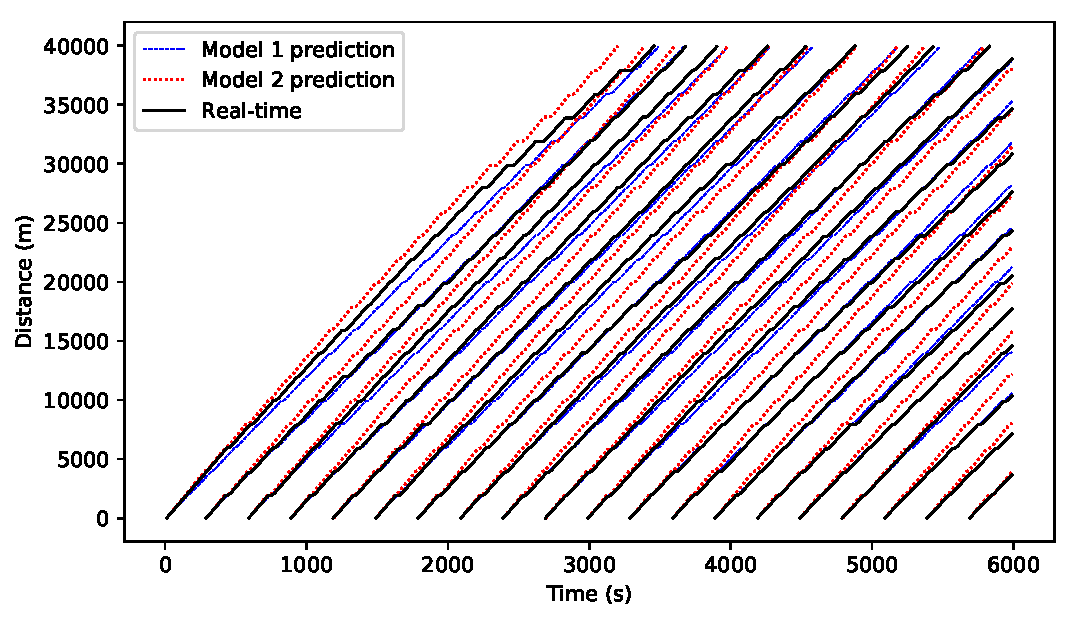
\includegraphics[width=\textwidth]{Figures/Fig_do_nothing_static.pdf}
    \caption{Prediction results from doing nothing scenario}
    \label{fig:do_nothing}
\end{figure}

Both Model 1 and Model 2 poorly predict the trajectories \DIFaddbegin \DIFadd{of the `real' buses}\DIFaddend . This is expected because the models do not have the optimal parameters to \DIFdelbegin \DIFdel{explain }\DIFdelend \DIFaddbegin \DIFadd{capture }\DIFaddend the bus route operations. \DIFdelbegin \DIFdel{Figure \ref{fig:do_nothing} shows the need to optimise the models with data, which we will address in the next subsection. }\DIFdelend \DIFaddbegin \DIFadd{This will be remedied in the following section. }\todo{This is good, but it also needs a single measure of error that can be used to quantify the differences across the different experiments. I usually use (S)RMSE or R2, but they're not necessarily the best so you choose one :-) Which one did you show me on the train?}
\DIFaddend 

\subsection{Parameter calibration}

\DIFdelbegin %DIFDELCMD < \todo[inline]{Here we use the two calibrated models to predict the bus locations and evaluate the results against the synthetic 'real-time' GPS data. We will show that both model still predict poorly without data assimilation, they after calibration they actual produce pretty similar prediction because both models converged to some 'optimal' value of parameters} 
%DIFDELCMD < 

%DIFDELCMD < %%%
\DIFdelend Model 1 and Model 2 are calibrated using Cross-Entropy Method, as described in Section \ref{s:calibration}. The two calibrated models are used to predict the bus locations at each time step $t$, which can be compiled to trajectories\DIFdelbegin \DIFdel{, similar to the previous 'doing nothing' scenario}\DIFdelend . Figure \ref{fig:calibration} shows the comparison between \DIFaddbegin \DIFadd{the predictions from }\DIFaddend Model 1 and Model 2 \DIFdelbegin \DIFdel{'s prediction }\DIFdelend versus the synthetic \DIFdelbegin \DIFdel{'}\DIFdelend \DIFaddbegin \DIFadd{`}\DIFaddend real-time' GPS data. \DIFaddbegin \DIFadd{Although they are an improvement on the un-calibrated versions (as expected), stochasticity in the `real' bus operations means that the simulated bus routes still diverge considerable from the real ones.
}\DIFaddend 

\begin{figure}[htb]
    \centering
    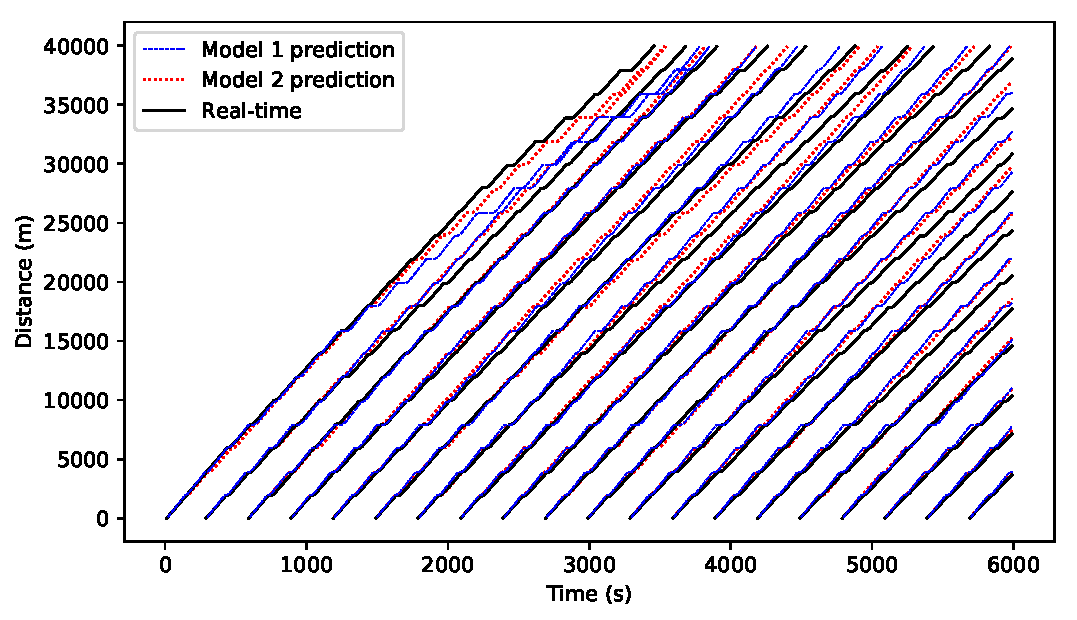
\includegraphics[width=\textwidth]{Figures/Fig_calibration.pdf}
    \caption{Prediction results after parameter calibration}
    \label{fig:calibration}
\end{figure}

\DIFdelbegin \DIFdel{There are two clear patterns that can be 
}%DIFDELCMD < 

%DIFDELCMD < %%%
\DIFdelend \subsection{Combination of parameter calibration and data assimilation (DA)}

\todo[inline]{Here we will show the prediction result after data assimilation. As can be seen in figure \ref{fig:calibration_plus_PF}, the results are better compared to \ref{fig:calibration}, but there are still large errors for later services. 

The figure below show the scenario where the dynamic change rate $\xi$ is 10\%. We will see that this is too much of a change and will find a point where the method will work} 

\DIFaddbegin \DIFadd{Figure~\ref{fig:calibration_plus_PF} illustrates the results after the models have been calibrated }\textit{\DIFadd{and}} \DIFadd{have `real-time' data incorporated (assimilated) into them during runtime.
}

\DIFaddend \begin{figure}[htb]
    \centering
    \includegraphics[width=\textwidth]{Figures/Fig_PF_300.pdf}
    \caption{Prediction results after parameter calibration and Particle Filtering}
    \label{fig:calibration_plus_PF}
\end{figure}

\subsection{Sensitivity analysis}

\todo[inline]{This is a systematic evaluation of the method against different value of stochasticity and dynamicity} 


  
    
    

\section{Conclusion\DIFaddbegin \label{s:conclusion}\DIFaddend }


\section{Acknowledgement}
This work has been supported by a European Research Council (ERC) Starting Grant (757455), a UK Economic and Social Research Council (ESRC) Future Research Leaders grant (ES/L009900/1) and a ESRC/Alan Turing Joint Fellowship (ES/R007918/1).

\bibliographystyle{apa}
\begin{thebibliography}{}

\bibitem[\protect\astroncite{Balmer et~al.}{2009}]{balmer2009matsim}
Balmer, M., Rieser, M., Meister, K., Charypar, D., Lefebvre, N., and Nagel, K.
  (2009).
\newblock Matsim-t: Architecture and simulation times.
\newblock In {\em Multi-agent systems for traffic and transportation
  engineering}, pages 57--78. IGI Global.

\bibitem[\protect\astroncite{Bertini and
  El-Geneidy}{2004}]{bertini2004modeling}
Bertini, R.~L. and El-Geneidy, A.~M. (2004).
\newblock Modeling transit trip time using archived bus dispatch system data.
\newblock {\em Journal of transportation engineering}, 130(1):56--67.

\bibitem[\protect\astroncite{Bin et~al.}{2006}]{bin2006bus}
Bin, Y., Zhongzhen, Y., and Baozhen, Y. (2006).
\newblock Bus arrival time prediction using support vector machines.
\newblock {\em Journal of Intelligent Transportation Systems}, 10(4):151--158.

\bibitem[\protect\astroncite{Carpenter et~al.}{1999}]{carpenter1999improved}
Carpenter, J., Clifford, P., and Fearnhead, P. (1999).
\newblock Improved particle filter for nonlinear problems.
\newblock {\em IEE Proceedings-Radar, Sonar and Navigation}, 146(1):2--7.

\bibitem[\protect\astroncite{Carrassi et~al.}{2018}]{carrassi_data_2018}
Carrassi, A., Bocquet, M., Bertino, L., and Evensen, G. (2018).
\newblock Data assimilation in the geosciences: {{An}} overview of methods,
  issues, and perspectives.
\newblock {\em Wiley Interdisciplinary Reviews: Climate Change}, 9(5):e535.

\bibitem[\protect\astroncite{Cats et~al.}{2010}]{cats2010mesoscopic}
Cats, O., Burghout, W., Toledo, T., and Koutsopoulos, H. (2010).
\newblock Mesoscopic modeling of bus public transportation.
\newblock {\em Transportation Research Record: Journal of the Transportation
  Research Board}, (2188):9--18.

\bibitem[\protect\astroncite{Chien et~al.}{2002}]{chien2002dynamic}
Chien, S. I.-J., Ding, Y., and Wei, C. (2002).
\newblock Dynamic bus arrival time prediction with artificial neural networks.
\newblock {\em Journal of Transportation Engineering}, 128(5):429--438.

\bibitem[\protect\astroncite{Chowdhury and Desai}{2000}]{chowdhury2000steady}
Chowdhury, D. and Desai, R.~C. (2000).
\newblock Steady-states and kinetics of ordering in bus-route models:
  connection with the nagel-schreckenberg model.
\newblock {\em The European Physical Journal B-Condensed Matter and Complex
  Systems}, 15(2):375--384.

\bibitem[\protect\astroncite{Crooks and Wise}{2013}]{crooks_gis_2013}
Crooks, A.~T. and Wise, S. (2013).
\newblock {{GIS}} and agent-based models for humanitarian assistance.
\newblock {\em Computers, Environment and Urban Systems}, 41:100--111.

\bibitem[\protect\astroncite{Eicker et~al.}{2014}]{eicker2014calibration}
Eicker, A., Schumacher, M., Kusche, J., D{\"o}ll, P., and Schmied, H.~M.
  (2014).
\newblock Calibration/data assimilation approach for integrating grace data
  into the watergap global hydrology model (wghm) using an ensemble kalman
  filter: First results.
\newblock {\em Surveys in Geophysics}, 35(6):1285--1309.

\bibitem[\protect\astroncite{Epstein and Axtell}{1996}]{epstein_growing_1996}
Epstein, J. and Axtell, R. (1996).
\newblock {\em Growing {{Artificial Societies}}: {{Social Science}} from the
  {{Bottom Up}}}.
\newblock {Brookings Institution Press}.

\bibitem[\protect\astroncite{Grazzini et~al.}{2017}]{grazzini_bayesian_2017}
Grazzini, J., Richiardi, M.~G., and Tsionas, M. (2017).
\newblock Bayesian estimation of agent-based models.
\newblock {\em Journal of Economic Dynamics and Control}, 77:26--47.

\bibitem[\protect\astroncite{Hans et~al.}{2015}]{hans2015real}
Hans, E., Chiabaut, N., Leclercq, L., and Bertini, R.~L. (2015).
\newblock Real-time bus route state forecasting using particle filter and
  mesoscopic modeling.
\newblock {\em Transportation Research Part C: Emerging Technologies},
  61:121--140.

\bibitem[\protect\astroncite{Harvey}{1990}]{harvey1990forecasting}
Harvey, A.~C. (1990).
\newblock {\em Forecasting, structural time series models and the Kalman
  filter}.
\newblock Cambridge university press.

\bibitem[\protect\astroncite{Heppenstall
  et~al.}{2007}]{heppenstall_genetic_2007}
Heppenstall, A.~J., Evans, A., and Birkin, M.~H. (2007).
\newblock Genetic algorithm optimisation of an agent-based model for simulating
  a retail market.
\newblock {\em Environment and Planning B: Planning and Design}, 34:1051--1070.
\newblock Cited by 0018.

\bibitem[\protect\astroncite{Hill}{2003}]{hill2003numerical}
Hill, S.~A. (2003).
\newblock Numerical analysis of a time-headway bus route model.
\newblock {\em Physica A: Statistical Mechanics and its Applications},
  328(1):261--273.

\bibitem[\protect\astroncite{Huijberts}{2002}]{huijberts2002analysis}
Huijberts, H. (2002).
\newblock Analysis of a continuous car-following model for a bus route:
  existence, stability and bifurcations of synchronous motions.
\newblock {\em Physica A: Statistical Mechanics and its Applications},
  308(1):489--517.

\bibitem[\protect\astroncite{Jiang et~al.}{2003}]{jiang2003realistic}
Jiang, R., Hu, M.-B., Jia, B., and Wu, Q.-S. (2003).
\newblock Realistic bus route model considering the capacity of the bus.
\newblock {\em The European Physical Journal B-Condensed Matter and Complex
  Systems}, 34(3):367--372.

\bibitem[\protect\astroncite{Kalnay}{2003}]{kalnay_atmospheric_2003}
Kalnay, E. (2003).
\newblock {\em Atmospheric {{Modeling}}, {{Data Assimilation}} and
  {{Predictability}}}.
\newblock {Cambridge University Press}.

\bibitem[\protect\astroncite{Khosravi et~al.}{2011}]{khosravi2011prediction}
Khosravi, A., Mazloumi, E., Nahavandi, S., Creighton, D., and Van~Lint, J.
  (2011).
\newblock Prediction intervals to account for uncertainties in travel time
  prediction.
\newblock {\em IEEE Transactions on Intelligent Transportation Systems},
  12(2):537--547.

\bibitem[\protect\astroncite{Kieu and Cai}{2018}]{kieu2018stochastic}
Kieu, L.~M. and Cai, C. (2018).
\newblock Stochastic collective model of public transport passenger arrival
  process.
\newblock {\em IET Intelligent Transport Systems}, 12(9).

\bibitem[\protect\astroncite{Lewis et~al.}{2006}]{lewis_dynamic_2006}
Lewis, J.~M., Lakshmivarahan, S., and Dhall, S. (2006).
\newblock {\em Dynamic {{Data Assimilation}}: {{A Least Squares Approach}}}.
\newblock {Cambridge University Press}, Cambridge.

\bibitem[\protect\astroncite{Lewis and Shedler}{1979}]{lewis1979simulation}
Lewis, P.~W. and Shedler, G.~S. (1979).
\newblock Simulation of nonhomogeneous poisson processes by thinning.
\newblock {\em Naval research logistics quarterly}, 26(3):403--413.

\bibitem[\protect\astroncite{Li et~al.}{2011}]{li2011cloud}
Li, Z., Chen, C., and Wang, K. (2011).
\newblock Cloud computing for agent-based urban transportation systems.
\newblock {\em IEEE Intelligent Systems}, 26(1):73--79.

\bibitem[\protect\astroncite{Lloyd et~al.}{2016}]{lloyd_exploring_2016}
Lloyd, D. J.~B., Santitissadeekorn, N., and Short, M.~B. (2016).
\newblock Exploring data assimilation and forecasting issues for an urban crime
  model.
\newblock {\em European Journal of Applied Mathematics}, 27(Special Issue
  03):451--478.

\bibitem[\protect\astroncite{Luo et~al.}{2012}]{luo2012realistic}
Luo, Y.-J., Jia, B., Li, X.-G., Wang, C., and Gao, Z.-Y. (2012).
\newblock A realistic cellular automata model of bus route system based on open
  boundary.
\newblock {\em Transportation Research Part C: Emerging Technologies},
  25:202--213.

\bibitem[\protect\astroncite{Macal and North}{2005}]{macal_tutorial_2005}
Macal, C.~M. and North, M.~J. (2005).
\newblock Tutorial on {{Agent}}-{{Based Modelling}} and {{Simulation}}.
\newblock In Kuhl, M.~E., Steiger, N.~M., Armstrong, F.~B., and Joines, J.~A.,
  editors, {\em Proceedings of the 2005 {{Winter Simulation Conference}}},
  pages 2--15. {Institute Of Electrical And Electronics Engineers}, Piscataway,
  NJ.

\bibitem[\protect\astroncite{Malleson et~al.}{2014}]{malleson_optimising_2014}
Malleson, N., See, L., Evans, A., and Heppenstall, A. (2014).
\newblock Optimising an {{Agent}}-{{Based Model}} to {{Explore}} the
  {{Behaviour}} of {{Simulated Burglars}}.
\newblock In Dabbaghian, V. and Mago, V.~K., editors, {\em Theories and
  {{Simulations}} of {{Complex Social Systems}}}, number~52 in Intelligent
  Systems Reference Library, pages 179--204. {Springer Berlin Heidelberg}.

\bibitem[\protect\astroncite{Meinhold and
  Singpurwalla}{1983}]{meinhold1983understanding}
Meinhold, R.~J. and Singpurwalla, N.~D. (1983).
\newblock Understanding the kalman filter.
\newblock {\em The American Statistician}, 37(2):123--127.

\bibitem[\protect\astroncite{Nagatani}{2000}]{nagatani2000kinetic}
Nagatani, T. (2000).
\newblock Kinetic clustering and jamming transitions in a car-following model
  for bus route.
\newblock {\em Physica A: Statistical Mechanics and its Applications},
  287(1):302--312.

\bibitem[\protect\astroncite{Nagatani}{2001}]{nagatani2001bunching}
Nagatani, T. (2001).
\newblock Bunching transition in a time-headway model of a bus route.
\newblock {\em Physical Review E}, 63(3):036115.

\bibitem[\protect\astroncite{O'loan et~al.}{1998}]{o1998jamming}
O'loan, O., Evans, M., and Cates, M. (1998).
\newblock Jamming transition in a homogeneous one-dimensional system: The bus
  route model.
\newblock {\em Physical Review E}, 58(2):1404.

\DIFaddbegin \bibitem[\protect\astroncite{Oloo and Wallentin}{2017}]{oloo_adaptive_2017}
\DIFadd{Oloo, F. and Wallentin, G. (2017).
}\newblock \DIFadd{An }{{\DIFadd{Adaptive Agent}}}\DIFadd{-}{{\DIFadd{Based Model}}} \DIFadd{of }{{\DIFadd{Homing Pigeons}}}\DIFadd{: }{{\DIFadd{A
  Genetic Algorithm Approach}}}\DIFadd{.
}\newblock {\em \DIFadd{ISPRS International Journal of Geo-Information}}\DIFadd{, 6(1):27.
}

\DIFaddend \bibitem[\protect\astroncite{Oremland and
  Laubenbacher}{2014}]{oremland_optimization_2014}
Oremland, M. and Laubenbacher, R. (2014).
\newblock Optimization of {{Agent}}-{{Based Models}}: {{Scaling Methods}} and
  {{Heuristic Algorithms}}.
\newblock {\em Journal of Artificial Societies and Social Simulation}, 17(2).

\bibitem[\protect\astroncite{Pennisi et~al.}{2008}]{pennisi_optimal_2008}
Pennisi, M., Catanuto, R., Pappalardo, F., and Motta, S. (2008).
\newblock Optimal vaccination schedules using simulated annealing.
\newblock {\em Bioinformatics}, 24(15):1740--1742.

\bibitem[\protect\astroncite{Ren et~al.}{2009}]{ren_agentbased_2009}
Ren, C., Yang, C., and Jin, S. (2009).
\newblock Agent-{{Based Modeling}} and {{Simulation}} on {{Emergency
  Evacuation}}.
\newblock In Akan, O., Bellavista, P., Cao, J., Dressler, F., Ferrari, D.,
  Gerla, M., Kobayashi, H., Palazzo, S., Sahni, S., Shen, X.~S., Stan, M.,
  Xiaohua, J., Zomaya, A., Coulson, G., and Zhou, J., editors, {\em Complex
  {{Sciences}}}, volume~5, pages 1451--1461. {Springer Berlin Heidelberg},
  Berlin, Heidelberg.

\bibitem[\protect\astroncite{Rubinstein}{1999}]{rubinstein1999cross}
Rubinstein, R. (1999).
\newblock The cross-entropy method for combinatorial and continuous
  optimization.
\newblock {\em Methodology and computing in applied probability},
  1(2):127--190.

\bibitem[\protect\astroncite{Schoenharl and
  Madey}{2011}]{schoenharl_design_2011}
Schoenharl, T. and Madey, G. (2011).
\newblock Design and {{Implementation}} of {{An Agent}}-{{Based Simulation}}
  for {{Emergency Response}} and {{Crisis Management}}.
\newblock {\em Journal of Algorithms \& Computational Technology},
  5(4):601--622.

\bibitem[\protect\astroncite{Schutte}{2010}]{schutte_optimization_2010}
Schutte, S. (2010).
\newblock Optimization and {{Falsification}} in {{Empirical Agent}}-{{Based
  Models}}.
\newblock {\em Journal of Artificial Societies and Social Simulation}, 13(1).

\bibitem[\protect\astroncite{Talagrand}{1991}]{talagrand_use_1991}
Talagrand, O. (1991).
\newblock The {{Use}} of {{Adjoint Equations}} in {{Numerical Modelling}} of
  the {{Atmospheric Circulation}}.
\newblock In Griewank, A. and Corliss, G.~F., editors, {\em Automatic
  {{Differentiation}} of {{Algorithms}}: {{Theory}}, {{Implementation}}, and
  {{Application}}}, pages 169--180. {SIAM}, Philadelphia, PA.

\bibitem[\protect\astroncite{Tang et~al.}{2012}]{Tang2012}
Tang, T., Shi, Y., Wang, Y., and Yu, G. (2012).
\newblock A bus-following model with an on-line bus station.
\newblock {\em Nonlinear Dynamics}, 70(1):209--215.

\bibitem[\protect\astroncite{Toledo et~al.}{2010}]{toledo2010mesoscopic}
Toledo, T., Cats, O., Burghout, W., and Koutsopoulos, H.~N. (2010).
\newblock Mesoscopic simulation for transit operations.
\newblock {\em Transportation Research Part C: Emerging Technologies},
  18(6):896--908.

\bibitem[\protect\astroncite{TRB}{2013}]{kfh2013transit}
TRB (2013).
\newblock Transit capacity and quality of service manual.
\newblock {\em Transit Cooperative Highway Research Program (TCRP) Report 165}.

\bibitem[\protect\astroncite{Wang and Hu}{2015}]{wang_data_2015}
Wang, M. and Hu, X. (2015).
\newblock Data assimilation in agent based simulation of smart environments
  using particle filters.
\newblock {\em Simulation Modelling Practice and Theory}, 56:36--54.

\bibitem[\protect\astroncite{Ward et~al.}{2016}]{ward_dynamic_2016}
Ward, J.~A., Evans, A.~J., and Malleson, N.~S. (2016).
\newblock Dynamic calibration of agent-based models using data assimilation.
\newblock {\em Royal Society Open Science}, 3(4).

\end{thebibliography}
 % Please set the right name for your bib file
\DIFaddbegin 



\end{document}